\documentclass[a4paper,titlepage]{report}

\usepackage{t1enc}
\usepackage[pdftex]{graphicx}
\usepackage{times}
\usepackage{a4wide}
\usepackage{hyperref}
\pdfcompresslevel=9
\usepackage{fancyvrb}
\usepackage{multind}

\makeindex{CmdFlags}

\parskip 5pt plus 3pt minus 2pt 

\newcommand{\EuGene}{\textsc{EuG\`ene}}
% comment one of the above line to hide or not the developpers documentation
%\newcommand{\shrink}[1]{}   % hide text
\newcommand{\shrink}[1]{#1} % no effect

\author{Philipe Bardou \and Marie-Jos\'ee Cros \and Sylvain Foissac \and J\'erome Gouzy \and Annick Moisan \and C\'eline Noirot \and Erika Sallet \and Thomas Schiex \\ Applied Mathematics and Computer Science Dept.\\ INRA Toulouse, France}

\def\abstractname{Overview}
\setcounter{tocdepth}{3}
\setcounter{secnumdepth}{3}

\title{\EuGene: an open gene finder for eukaryotes}

\begin{document}
\maketitle
\tableofcontents

\begin{abstract}
  \EuGene\ is a sophisticated open gene finder for eukaryotic
  organisms. It has been developped thanks to funding by INRA
  (permanent scientists and engineers), G\'enoplante and the french
  ministry of research (with one PhD student). It generates text, HTML
  and graphical outputs.
  
  \EuGene\ uses a graph based model to predict genes that covers both
  HMM based or more complex Bayesian net based or Conditional Markov Field probabilistic
  predictions. The model is fixed but complex (with 43 different
  states) and covers Exon, Intron, UTR, UTR introns\ldots each with a
  possible explicit distribution on length. The prediction itself
  relies on an optimal linear time and space algorithm for prediction.
  
  Even if the gene model is fixed, the sources of information taken
  into account be \EuGene\ for prediction are extremely varied and can
  be easily extended by creating so-called plugins. Currently,
  \EuGene\ can use around 30 different plugins integrating statistical
  information (Markov models at DNA or amino acid level, WAM, Support
  Vector machine based signal prediction\ldots), similarity information
  (Est, cDNA, proteins) and homology (exon conservation). It can also
  integrate predictions from other gene predictors if needed.
  
  In order to integrate all this information, \EuGene\ does not use
  maximum likelihood estimation for all parameters but parameters
  optimized by maximum of prediction quality on expertized data sets (minimizing
  empirical risk on a given dataset).

  The software called \texttt{eugene} is written in C++ and is distributed 
  under the artistic license.
 \end{abstract}

\chapter{Quick Start}

\section{Annoting a sequence}
Here is a small example based on the \texttt{SYNO\_ARATH.fasta} sequence.
For reference information on the software, see chapter 2.

In order to first collect information on the sequence (splice sites,
translation start predictions\ldots) we will have to use the
\texttt{getsites4eugene.pl} script. This script directly queries the
Netgene2, SPlicePredictor and NetStart web servers. Alternatively, if
you have installed these programs locally, you can use the
\texttt{lgetsites4eugene.pl} script (you must modify it and indicate
the paths to the executables). 

\begin{Verbatim}[fontsize=\scriptsize]
> ./getsites4eugene.pl Sequences/SYNO_ARATH.fasta 
started on sam dec 7 13:44:35 CET 2002

processing Sequences/SYNO_ARATH.fasta

NetStart [2*1 request(s)]: F1..R1..done
NetGene2 [1   request(s)]: 1..FR..done
SplicePredictor: done
finished on sam dec 7 13:47:14 CET 2002
\end{Verbatim}

The script creates the files that contains information about the
sequence in the same directory as the fasta file itself. The
extensions used are \texttt{.splices} for NetGene2, \texttt{.spliceP}
for SplicePredictor, \texttt{.starts} for NetStart (in each case, a
\texttt{R} is added for the reverse strand). 

We are now ready to use \EuGene\ on this sequence. Because the
sequence lacks context around the CDS of the gene, we inform \EuGene\ 
that the prediction should start and end in intergenic mode using the
\texttt{-s} flag. This behavior can also be controlled by all the
\texttt{Prior} parameters in the program parameter file (see
section~\ref{param}).

\EuGene\ produce two kind of output: textual and graphical. To manage this outputs
several options could be use. Two of them (more details see chapter 2):
\begin{itemize}
\item \texttt{-p a|d|g|h|l|s|o}: if we want, we may ask for multiple textual output. For example an HTML output
and an GFF output using the \texttt{-phg} flag. Two files will be created '\texttt{SYNO\_ARATH.html}'
and '\texttt{SYNO\_ARATH.gff}'. \texttt{-po} allows to print prediction on stdout.
\item \texttt{-g}: activates the graphical output (with \texttt{-ph} flag \texttt{-g} is on).\\
\end{itemize}

\begin{Verbatim}[fontsize=\scriptsize]
EXECUTION_TRACE1
\end{Verbatim}

\section{Using transcribed sequences}

If you want to exploit similarities with cDNA/EST sequences, you have to inform \EuGene\ of existing similarities. These similarities
should be available in a file with the \texttt{.est} extension. The
format of this file is described in the \texttt{Est} plugin
section~\ref{plugest}. It can easily be created from an existing FASTA
databank of EST and cDNA using a patched version of \texttt{sim4}. The
patch is provided with \EuGene.

\begin{Verbatim}[fontsize=\scriptsize]
> sim4 Sequences/SYNO_ARATH.fasta cDNA A=6 > seqs/SYNO_ARATH.fasta.est
\end{Verbatim}

With an old dbEST databank completed with the cDNA databank PlantGene,
we get the following file:

\begin{Verbatim}[fontsize=\scriptsize]
> cat Sequences/SYNO_ARATH.fasta.est
    32    421 1844 0 0 ATAJ644    1  390
   514    582 1844 0 0 ATAJ644  391  459
   699    809 1844 0 0 ATAJ644  460  570
   914   1018 1844 0 0 ATAJ644  571  675
  1271   1408 1844 0 0 ATAJ644  676  813
  1522   1602 1844 0 0 ATAJ644  814  894
  1694   1771 1844 0 0 ATAJ644  895  972
  1853   1921 1844 0 0 ATAJ644  973 1041
  2014   2088 1844 0 0 ATAJ644 1042 1116
  2181   2264 1844 0 0 ATAJ644 1117 1200
  2360   2446 1844 0 0 ATAJ644 1201 1287
  2712   2882 1844 0 0 ATAJ644 1288 1458
  2966   3092 1844 0 0 ATAJ644 1459 1585
  3189   3447 1844 0 0 ATAJ644 1586 1844
    32    375 347 0 0 N97006    1  347
  3099   3379 297 0 0 AV525988   51  347
  3071   3092 256 0 1 AI994358    1   22
  3189   3421 256 0 1 AI994358   23  256
   658    672 61 0 1 AV521563    1   14
   765    813 61 0 1 AV521563   15   61
\end{Verbatim}

We can now ask \EuGene\ for a new prediction, including this new
evidence using the \texttt{-d} flag (equivalently, the \texttt{Est}
plugin can be activated by modifying \EuGene\ parameter file).  When
evidence from transcribed sequences is available, \EuGene\ will
automatically report in the last column of its output the percentage
of bases of the element (exon, UTR\ldots) which is consistent with the
available evidence. Here, the gene is almost completely covered by the
available transcribed sequences. The \texttt{Est} plugin also mentions
if transcribed sequences are rejected and why. The information from
two transcribed sequences is rejected. The first one because no splice
site has been found near one of the intron border detected by the EST,
another one because it was inconsistent with a sequence considered as
more reliable.

\begin{Verbatim}[fontsize=\scriptsize]
EXECUTION_TRACE2
\end{Verbatim}

An additional postprocessing can be requested to the plugin using the
\texttt{-E} flag. For each gene predicted, the plugin will analyze
each transcribed sequence matching the gene and report its consistency
with the prediction in '\texttt{SYNO\_ARATH.misc\_info}' file.

\begin{Verbatim}[fontsize=\scriptsize]
EXECUTION_TRACE3
\end{Verbatim}

% TO UPDATE: THOMAS
%One can see that 2 of the 5 transcribed sequences have been filtered.
%\texttt{ATAJ644} is an almost full-length cDNA. It covers almost all
%the gene, from the position after the ATG to the 3'UTR. At the end,
%for each gene predicted, a summary reports that the CDS predicted is
%supported by 3273 over 3276 bases (the ATG is missing in all
%trannscripts). The transcribed sequence predicted (including the UTR)
%is supported for 3416 of its 3444 bases.

\section{Using protein similarities}

If one wants also to exploit similarities with homologous proteins, a
similar file format can be used (see the corresponding plugin). The
plugin can analyze similarities from several databases, each being
associated with a specific ``level''. For each level, a confidence is
defined in \EuGene's parameter file. Usually, 3 databases are used:
SwissProt, PIR and TrEMBL (from the highest confidence to the
lowest). Each collection of similarity is stored in a file with an
extension \texttt{.blast} followed by the level of the database 
(\texttt{.blast0}, \texttt{.blast1}, ..., \texttt{.blast9}).  The
script used create these files from the output of NCBI-BLASTX is
copyrighted and is therefore not distributed with \EuGene. It is not
difficult to design another one. Here is an extract from
\texttt{SYNO\_ARATH.fasta.blast0}:

\begin{Verbatim}[fontsize=\scriptsize]
2820 2861 36 3e-08 +3  sp_O07683_SYD_HALSA; 335 348
2972 3088 41 3e-08 +2  sp_O07683_SYD_HALSA; 359 397
3185 3298 113 3e-08 +2  sp_O07683_SYD_HALSA; 398 435
353 418 45 2e-13 +2  sp_O24822_SYD_HALVO; 13 34
1850 1915 67 2e-13 +2  sp_O24822_SYD_HALVO; 202 223
2775 2858 72 2e-13 +3  sp_O24822_SYD_HALVO; 318 345
3191 3280 104 2e-13 +2  sp_O24822_SYD_HALVO; 397 426
353 418 51 7e-12 +2  sp_O26328_SYD_METTH; 21 42
1271 1414 70 7e-12 +2  sp_O26328_SYD_METTH; 141 188
1850 1954 62 7e-12 +2  sp_O26328_SYD_METTH; 210 244
3191 3280 93 7e-12 +2  sp_O26328_SYD_METTH; 401 430
\end{Verbatim}

To exploit this information, the \texttt{-b} flag must be used,
optionally followed by the set of levels to be exploited
(``\texttt{012}'' means level 0, 1 and 2).  We start \EuGene\ and ask
for both EST and proteic similarities analysis. We again enforce the
use of an intergenic mode on the beginning and end of the sequence.
And similar to the EST, an additional postprocessing can be requested
to the plugin using the \texttt{-B} flag.

\begin{Verbatim}[fontsize=\scriptsize]
EXECUTION_TRACE4
\end{Verbatim}

Other plugins are described in the reference section of this document.

\newpage
\chapter{Reference documentation}

To be executed, \EuGene\ needs at least one file: this is the
so-called parameter file.  \EuGene\ behavior is entirely controlled
by a set of parameters whose default values are available in this
file. These default values can be altered by editing this file or for
some values through flags in the command line (such as \texttt{-d},
see the quick start chapter). Command line flags override any value in the parameter
file. The name of the parameter file that \EuGene\ seeks is obtained
by adding the suffix ``\texttt{.par}'' to the name of the \EuGene\ 
command itself.  As it is distributed, \EuGene\ command's name is
\texttt{eugene} and accordingly the parameter file is
\texttt{eugene.par}. If at some point you want to use several
different parameter files, you can simply use symbolic links to the
\texttt{eugene} binary executable. Using a symbolic link, with a
specific name to call \EuGene\ will enable you to load a different
parameter file whose name is derived from the symbolic link name by
ading `\texttt{`.par}'' The parameter file is first sought in the
local directory.  If this fails, the value of the environment variable
\texttt{EUGENEDIR} is used as a second possible path.

\EuGene\ gathers all informations on the FASTA sequences through
so-called ``plugins'' also called ``sensors''. A plugin is a small
software component that can be dynamically loaded and that can inform
\EuGene\ about likely exonic, intronic, utr, intergenic regions and
about signals in the sequence (either splice sites, translation starts
and stops, transcription starts and stops and possible frameshifts).
Plugins can typically embody Markov models (that characterize exonic,
intronic\ldots regions) or splice site detectors or others.  Available
sensors are stored in the \texttt{PLUGINS} directory and are
dynamically loaded by \EuGene\ according to the parameters.

The typical call to \EuGene\ is:

\begin{Verbatim}[fontsize=\small]
eugene <fasta files>
\end{Verbatim}

where each FASTA file contains one single DNA sequence. In this case,
the first action of \EuGene\ is to seek and load the parameter file.
All the parameters in this file are either used by \EuGene\ or by the
plugins. Each plugin may have its own parameters. The following
section describes all the parameters used by \EuGene. Information
about the parameters used by plugins is provided in each plugin
section (see section~\ref{plug}).

\section{\EuGene's general parameters}
\label{param}

Here is a list of all the parameters not related to a plugin which control \EuGene's
behavior. When a command line flag exists that can modify the
corresponding parameter, it is indicated.  All the parameters that
control \EuGene\'s behavior are available in the parameter file. This
file has a relatively strict formatting. Each line can either be a
comment line (the first character in the line must be a \verb # ) or a
parameter definition. Empty lines are not allowed. A parameter
definition is composed of two strings of character. The first one is
the name of the parameter, the second is its value. Everything is case
sensitive. The definition order is not important.

\begin{itemize}
\item \texttt{EuGene.version}: specifies the \EuGene \ version. 
  After having load the parameter file, \EuGene \ checks
  that the parameter file version is consistent with the executable
  version.

\item \texttt{EuGene.organism}: name of the considered organism.
   
\item \texttt{EuGene.PluginsDir}: specify the location of the directory
  where plugins could be found (``\texttt{.so}'' files, sensor specific 
  models files); that is the path to the \texttt{PLUGINS} directory.
  
  \item \texttt{EuGene.sloppy}: in the default (non-sloppy) mode, 
  \EuGene\ will stop and abort if some needed parameters in the parameter
  file is missing. If the parameter is set to \texttt{1} then a simple warning
  is emitted. Not advised unless you know what you do.
  
\item \texttt{EuGene.ExonPrior}, \texttt{EuGene.IntronPrior},
  \texttt{EuGene.InterPrior}, \texttt{EuGene.FivePri\-mePrior},
  \texttt{EuGene.ThreePrimePrior}: prior on the initial/final state of
  prediction. The ``\texttt{-s}'' command line flag can override these
  priors by setting all the non intergenic priors to $0.0$. This
  forces \EuGene\ to start and and its prediction in intergenic mode.
  
\item \texttt{EuGene.InitExDist}, \texttt{EuGene.IntrExDist},
  \texttt{EuGene.TermExDist}, \texttt{EuGene.SnglExDist},
  \texttt{EuGene.IntronDist}, \texttt{EuGene.InterDist},
  \texttt{EuGene.5PrimeDist}, \texttt{EuGene.3PrimeDist}: \EuGene\ 
  can use explicit penalty distributions on the length of the elements
  predicted. This can be an initial exon, and intermediary exon, a
  terminal exon, a single exon gene, an intron an intergenic region, a
  5' UTR region or a 3' UTR region. Each parameter specifies the
  filename of an explicit penalty distribution file (see the following section). %TBD
  
\item \texttt{EuGene.SplicedStopPen}: indicates the penalty for
  predicting genes containing in-frame spliced STOPs. This is
  basically set to an infinite value in order to avoid prediction
  containing spliced STOPs but setting this to 0.0 can be useful for
  pseudo-gene prediction\ldots

\item \texttt{Output.RemoveFrags}: in the text output, remove any 
fragmentary gene prediction (missing ATG or STOP or both). The prediction
process is unchanged,  the prediction is just filtered. \index{CmdFlags}{[Remove fragmentary proteins] F}

\item \texttt{Output.truncate}: in the text output, each gene element
  predicted if prefixed by the FASTA sequence id (or the filename if
  no FASTA id is available). This is truncated to the number of
  caracters indicated. If set to 0 (or FALSE), the full id is used.

\item \texttt{Output.MinCDSLen}: any predicted gene whose CDS length
  in number of nucleotides is lower than this is filtered out from the
  output.

\item \texttt{Output.UTRtrim}: EuGene is natively capable of
  predicting UTR. If desired however, the UTR prediction of EuGene can
  be trimmed to be exactly consistent with the transcript evidence
  available as provided by the Est plugin. If no EST evidence is
  available, this means that all UTR predictions will be removed from
  the output.

\item \texttt{Output.stepid}: in the text output, step for numbering genes.

\item \texttt{Output.graph}: if set, requests graphical PNG output.
  This can also be set using the \texttt{-g} command line flag. \index{CmdFlags}{[eugene PNG graph required] g}
  The PNG filename is composed by the seq name (w/o the .fasta suffix) completed by
  the number of the figure + .png extension (possibly,
  start/end positions will be inserted too if -u/-v is used).
  
\item \texttt{Output.resx}, \texttt{Output.resy}: controls the
  horizontal and vertical resolution of the PNG images generated by
  \EuGene. 
  
\item \texttt{Output.gfrom}, \texttt{Output.gto}: respectively
  controls which part of the sequence is to be plotted (eg. for
  zooming). The default value for both is $-1$ which corresponds to
  the whole sequence. These parameters can also be set using the
  \texttt{-u} and \texttt{-v}. flags \index{CmdFlags}{[eugene PNG graph lower bound] u}
  \index{CmdFlags}{[eugene PNG graph higher bound] v}

\item \texttt{Output.glen}: controls the number of nucleotides that
  will appear on a single image. The value $-1$ corresponds to a
  default adaptative mechanism which plots min (6000,length to
  visualize). The ``length to visualize'' is computed from the value
  given to \texttt{Output.gfrom} and \texttt{Output.gto}.
  
\item \texttt{Output.golap}: controls how successives PNG images
  overlap. It must be set to the number of overlapping nucleotides
  between 2 successives PNG images. Default is $-1$ which
  heuristically determines this based on resolution and number of nuc.
  per image. This parameter can also be set using the \texttt{-c}
  command line flag. \index{CmdFlags}{[eugene PNG graph overlapping] c}
    
\item \texttt{Output.normopt}: indicates the way the score are
  normalized accross the possibles states (phase 1, 2, 3, -1, -2, -3,
  introns and intergenic states).
  \begin{itemize}
  \item 0: no normalization
  \item 1: normalize accross all states
  \item 2: normalize each coding phase w.r.t. to the non coding
    score only.
  \end{itemize}
  Default is 1. Does not affect prediction, only graphical output.

\item \texttt{Output.window}: sets the half-size of the smoothing
  window used to plot the scores.  Default is 48. This does not affect
  prediction, only graphical output. It can be set using the
  \texttt{-w} command line flag. \index{CmdFlags}{[eugene PNG graph smoothing window] w}

\item \texttt{Output.intron}: allows to print introns in the textual output.
  Default is 0 (no introns).
 
\item \texttt{Output.format}: controls the format of the textual
  outpout. May be \texttt{o} (stdout), \texttt{d} (detailed),
  \texttt{l} (long), \texttt{s} (short), \texttt{h} (html), \texttt{g}
  (gff) or \texttt{a} (araset format). Default is \texttt{l}. This can
  be overrided using the \texttt{-p} command line
  flag.\index{CmdFlags}{[eugene textual output format] p} \texttt{o}:
  print the prediction on stdout using the same format than
  \texttt{l}.  All the others print the prediction in files which name
  are composed by the name of the sequence file (w/o the extension
  .fasta, .tfa, .fsa or .txt) completed by \texttt{.egn.debug (d)},
  \texttt{.egn (l)}, \texttt{.egn.short (s)}, \texttt{.html (h)},
  \texttt{.gff (g)}, \texttt{.gff3 (g)} or \texttt{.egn.ara (a)}.
  Multiple format can be selected (\texttt{ohg} for example). When GFF
  is requested, both GFF1 and GFF3 are produced.
  
\item \texttt{Output.offset}: allows to offset the nucleotide position
  of the prediction.  That is, the prediction for nucleotide at
  position $i$ of the given sequence is printed as nucleotide $i+$ the
  offset. Useful to perform prediction on an extracted sequence
  without loosing the original position. Can also be set using the
  \texttt{-o} command line flag. \index{CmdFlags}{[eugene nucleotide position offset] o}
  
\item \texttt{Output.Prefix}: indicates the directory where all non
  stderr/stdout output (eg. PNG images, HTML and GFF files...) should go.
  Default is the current directory.
  \index{CmdFlags}{[eugene output directory] O}

\item \texttt{Gff3.SoTerm}: indicates the path where sofa (Sequence Ontology Feature Terms) terms are store.
  The path is relative to EUGENEDIR.

\item \texttt{Eval.offset}: using during the evaluation of a prediction. 
The prediction is compared with a reference (the real gene structure). 
The region in which compare the prediction and the reference is defined 
	as the reference positions +/- the offset.

\item \texttt{Fitness.wsng}, \texttt{Fitness.wsne}, 
\texttt{Fitness.wsnn}, \texttt{Fitness.wspg}, 
\texttt{Fitness.wspe}, \texttt{Fitness.wsspn}: 
indicate respectively the weight of the gene sensitivity, of the exon sensitivity, 
of the nucleotide sensitivity, of the gene specificity, of the exon specificity 
and of the nucleotide specificity in the fitness computing.
\end{itemize}

{\bf Specification of explicit penalty distributions on length}

As in semi-Markov models, \EuGene\ uses explicit distribution of
penalties on the length of all predicted elements. The dynamic
programming inside \EuGene\ garantees that \EuGene\ will run in linear
time and space in the length of the sequence in all cases.

The distributions handled by \EuGene\ are made of 3 components. First,
there is a region of forbidden length (minimum length), then a region
with an arbitrary penalty distribution, then a region with a linear
variation of the penalty. From a probabilitic point of view, this means
an exponential tail.

Although \EuGene\ is linear in time in the sequence length, it is also
typically linear in time in the sum of the size of the two first
regions. For the moment, all existing \EuGene\ instances use explicit
distributions with an empty arbitrary region (the distribution is just
a minimum length followed by an exponential tail).

Explicit distributions must be specified in distribution files. Each
line in a distribution file contains a length and a penalty. The first
length used specifies the minimum allowed length. Then each line
specifies a point of the explicit distribution. Linear interpolation
is used between points. Then the last length used specifies the start
of the linear tail. The last slope used becomes the slop of the linear
tail.

A
typical distribution file is given below:
\begin{Verbatim}
3 0.0
4 2.0
6 4.0
\end{Verbatim}

It specifies a minimum length of 3. We then have an explicit
distribution region with penalty 0.0 for 3, 2.0 for 4, 3.0 for 5
(linear interpolation), then 4.0 at 6. As this is the last point
and the slope is 1, the rest of the distribution will be linear
with slope 1.

\section{Splice variant prediction}

Since version 3.4, \EuGene\ allows to predict splice variants based purely on
experimental data (alternative transcripts observed through EST). The feature
is still experimental and is activated using the \texttt{-a} flag or 
equivalently by setting the parameter \texttt{AltEst.use} to 1 or TRUE.\index{CmdFlags}{[splice isoform prediction] a}

In this case, \EuGene\ will look for a file with the same name as the sequence
file and with a suffix '\texttt{.alt.est}'. This file has the same format as
the '\texttt{.est}' used by the Est pugin (see later) and contains information
about genomic region with high quality similarity with EST. The spliced 
alignment algorithm used to create this file should be of high quality, 
with clear exon-intron frontiers associated with splice sites (use for example
GeneSeqer or faster GenomeThreader).

\EuGene\ will analyze these EST and look for pairs of EST which are inconsistent
one with the other (there is one nucleotide mapped to an exon by one which is 
mapped to an intron/gap by the other). Each element of such a pair will be used 
to try to produce a prediction that follows the EST structure. If the prediction
is different from the optimal prediction, the gene variant structure will be
also output.

This feature is controlled by a number of parameters with the '\texttt{AltEst}'
prefix in the parameter file. The only parameters that you could change are the
parametrs regarding length thresholds, used for filtering (\texttt{AltEst.maxEstLength}, \texttt{AltEst.minEstLength}, \texttt{AltEst.maxIn}, \texttt{AltEst.minIn}, \texttt{AltEst.maxEx} and \texttt{AltEst.minEx} which speak for themselves.

Every alignement is also "trimmed" by an amount of \texttt{AltEst.exonucleasicLength} on the first and last hit to account for possible spurious short matches. If these hits are shorter than this amount, they are removed from the available data.

Using the sequence \texttt{At5g18830.fasta.genomicAJ011613.fasta} and the associated information found in
the \texttt{doc/Sequences/} directory, we can test this as follows:

\begin{Verbatim}[fontsize=\scriptsize]
EXECUTION_TRACE5
\end{Verbatim}

We can see that two predictions are produced for the same region. In this case, it is just one alternative splice site
that has been used for the exon number 8 in the gene.

\section{Plugins}
\label{plug}

Plugins are small software components that can be dynamically loaded
by \EuGene. Although it is completely transparent to the end-user,
every plugin loaded by \EuGene\ must be written in C++ and be a
subclass of the Sensor class. This class provides essentially four
methods:
\begin{itemize}
\item constructor: when instanciated, a plugin receives an instance number
  (specified in the parameter file) and a DNA sequence (instance of
  the \texttt{DNASeq} class). The instance number allows to load
  several identical plugins using different parameters. A plugin with
  a parameter \texttt{X} and instance number \texttt{n} will fetch
  parameter \texttt{X[n]} in the parameter file. On instanciation, the
  plugin should load all data needed to handle the sequence. If the
  plugin depends on optimizable parameters (parameters whose name is
  followed by a \texttt{*}), then the final configuration that may
  depend on these parameters must be postponed in the \texttt{Init}
  method. 
  
\item \texttt{Init}: receives as argument the sequence to process (an
  instance of the \texttt{DNASeq} class) and performs the extra
  initializations that depends on optimizable parameters values
  (parameters whose name is followed by a \texttt{*}).
  
\item \texttt{GiveInfo}: receives as argument the sequence to process
  (an instance of the \texttt{DNASeq} class), a position on the
  sequence and a \texttt{Data} instance. The \texttt{Data}
  data-structure can receive predictions on all signals and contents
  scores known to \EuGene.

\item \texttt{Plot}: receives as argument the sequence to process (an
  instance of the \texttt{DNASeq} class) and plots all the predictions
  made by the sensor.

\item \texttt{PostAnalyse}: receives as argument the prediction of
  \EuGene\ and may check it against its own prediction and report
  support or inconsistencies.
\end{itemize}

The \texttt{Plot} and \texttt{PostAnalyse} methods are often empty.
The \texttt{Init} is usually limited to the reloading of optimizable
parameters (see the source of the \texttt{Est} or \texttt{BlastX}
plugins for exceptions).

\subsection{Loading plugins}

When \EuGene\ starts, plugins are loaded and instanciated following
parameters in the parameter file. The \texttt{Sensor.*.use} may
activate or desactivate the corresponding sensor (which must be
available in the PLUGINS directory). If the parameter value is set to
\texttt{0} or \texttt{FALSE}, the plugin is not used. If the parameter
value is set to \texttt{1}, then a single instance of the plugin is
loaded. If the parameter is set to an integer value, then this number
of instances of the plugin are created.

Below is the list of minimum plugins which are activated by default by
the \emph{Arabidopsis thaliana} version of \EuGene.

\begin{Verbatim}
Sensor.Transcript.use   1
Sensor.EuStop.use       1
Sensor.NStart.use       1
Sensor.IfElse.use       1 (with 2 splice site prediction plugins)
Sensor.MarkovIMM.use    1
Sensor.MarkovConst.use  1
\end{Verbatim}  

Sensors are loaded and instanciated following an increasing order of
priorities. The priority of a given type of plugin is defined by the
value of the corresponding \texttt{Sensor.*} parameter. Here is an
example of actual priorities:

\begin{Verbatim}
Sensor.Transcript       1
Sensor.FrameShift       1
Sensor.IfElse           1
Sensor.EuStop           1       
Sensor.NStart           1       
Sensor.MarkovIMM        1 
Sensor.Est              30         
\end{Verbatim}

The \texttt{Sensor.Est} is loaded last because it has the highest
priority.  This is important since the sensor actually uses the
information provided by other sensors (splice site prediction sensors)
that then have to be loaded before.

Several instances of the same sensor can be loaded. Eg., if you are
dealing with an organism that has a large GC\% range, one may use
several \texttt{Sensor.MarkovIMM}. Imagine you want to use one model
for sequences who have a GC\% below 50 and another for higher GC\%.
This can be achieved by instaciating 2 such sensors. 

\begin{Verbatim}
Sensor.MarkovIMM        2
\end{Verbatim}

When these sensors will be instanciated, they will look for specific
parameters. The first instance will use the usual parameters or parameters 
followed by \texttt{[0]} for this plugin class, the second instance will use parameters 
followed by \texttt{[1]}.

\begin{Verbatim}
MarkovIMM.matname[0]    lowGC.mat 
MarkovIMM.minGC[0]      0
MarkovIMM.maxGC[0]      50
MarkovIMM.matname[1]    highGC.mat
MarkovIMM.minGC[1]      50
MarkovIMM.maxGC[1]      100
\end{Verbatim}

As the example show, it is equivalent to define the parameter
\texttt{MarkovIMM.matname[0]} (or any parameter followed by
\texttt{[0]} and the parameter \texttt{MarkovIMM.matname}.

\subsection{\texttt{GFF3 input documentation}} 

Since version 3.4b, Eugene allows for Gff3-compliant input and output.

\paragraph{GFF3 format}

See \texttt{http://www.sequenceontology.org/gff3.shtml} for details.
In a GF33 file, everything is line-based. The format of a line is:

\verb!<seqid> <source> <type> <start> <end> <score> <strand> <phase><attributes>!

The attributes column is composed of tags, some tags have predefined
meanings according to Gff3 specifications. These are the tags
\texttt{ID, Target, Ontology\_term}.  For Eugene, we define additional
specific attributes: \texttt{is\_full\_length, target\_length,
  target\_sequence, database, frame\_hit, frame\_hit, score\_hit}.

A new parameter is needed in \texttt{eugene.par}: 
\texttt{Gff3.SoTerms		cfg/sofa.obo}

It specifies the path relatively to EUGENEDIR of the file which contains
all SOFA codes. Currently we use the version 1.2 of 25:07:2007. In order
to create valid gff3 file, you have to use SOFA terms or codes.

The third column (type) of gff3 format must contain a term of SOFA,
program accept the id, name and synonyms.

Example of SOFA definition term :
\begin{Verbatim}
[Term]
id: SO:0000164
name: three_prime_splice_site
def: "The junction between the 3 prime end of an intron and 
the following exon." [http://www.ucl.ac.uk/~ucbhjow/b241/glossary.html]
subset: SOFA
synonym: "3' splice site" RELATED []
synonym: "acceptor" RELATED []
synonym: "acceptor splice site" EXACT []
synonym: "splice acceptor site" EXACT []
is_a: SO:0000162 ! splice_site
\end{Verbatim}

The accepted types in the third columns are:

\begin{itemize}
\item\texttt{ SO:0000164}
\item\texttt{ three\_prime\_splice\_site}
\item\texttt{ acceptor }
\item\texttt{ acceptor splice site or  acceptor\_splice\_site}
\item\texttt{ splice acceptor site or  splice\_acceptor\_site}
\end{itemize}

Each plugin has its own extension, in gff3 mode you just have to add '.gff3' after the native file name.
Example if plugin \texttt{SPred} is active with gff3 input format , it will expect 
a file named \texttt{file.SPred.gff3} ( instead of \texttt{file.SPred} in native mode)

We now descrive each plugin, its behavior and parameters.

\subsection{\texttt{Signal plugins}}
% Documentation of the EuStop sensor

\subsection{\texttt{Sensor.EuStop}}

\paragraph{Description}

This simple plugin predicts translation stops. It is able to deal with
noisy sequences and will eg. predict a possible stop on \texttt{TGN}.

The sensor is activated by setting the value TRUE for the parameter
\texttt{Sensor.EuStop.use} in the parameter file.

The penalty payed for using a Stop is defined by the
\texttt{EuStop.stopP} parameter.

Here is an example of EuStop parameters definition.
\begin{Verbatim}[fontsize=\small]
EuStop.stopP*           4.155   # Stop penalty
Sensor.EuStop.use       TRUE    # Use EuStop sensor
Sensor.EuStop           1       # Sensor priority
\end{Verbatim}

\paragraph{Input files format}

No input files  needed.

\paragraph{Filtering input information}

No filtering.

\paragraph{Integration of information}

In the case of non degenerated sequences, all predictions using a Stop
to end a terminal exon are given an extra \texttt{EuStop.stopP}
penalty. All predictions going through an in-phase Stop in an exonic
state receive an infinite penalty.

\paragraph{Post analyse}

No post analyse.

\paragraph{Graph}

Every predicted Stop is ploted as a small vertical red bar in the
corresponding phase.



% Documentation of the FrameShift sensor

\subsubsection{\texttt{Sensor.FrameShift}}

\paragraph{Description}

This plugin predicts possible frameshifts (either insertions or
deletions) at each position of the sequence with a uniform cost. The
parameters \texttt{FrameShift.Ins*} \texttt{FrameShift.Del*} give the
corresponding penalties.

The sensor is activated by either:
\begin{itemize}
\item the \texttt{-f} argument \index{CmdFlags}{[FrameShift activation] f}.
\item the value 1 for the parameter \texttt{Sensor.FrameShift.use} in
  the parameter file.
\end{itemize}

Here is an example of FrameShift parameters definition.
\begin{Verbatim}[fontsize=\small]
FrameShift.Ins*        1e999.0
FrameShift.Del*        1e999.0
Sensor.FrameShift.use  1     # Use FrameShift sensor
Sensor.FrameShift      1        # Sensor priority
\end{Verbatim}

\paragraph{Input files format}

No input files  needed.

\paragraph{Integration of information}

All predictions that use a frameshift (going from one coding phase to
another coding phase) are given an extra \texttt{FrameShift.Ins*} or
\texttt{FrameShift.Del*} penalty according to the phase change.

\paragraph{Post analyse}

No post analyse.

\paragraph{Graph}

Every predicted frameshift is plotted as a vertical red line that
connect the exonic prediction blocks in the 2 corresponding phase.



% Documentation of the GSplicer sensor

\subsection{\texttt{Sensor.GSplicer}}

\paragraph{Description}

The GSplicer sensor injects possible splice sites as predicted by the
\textsc{GeneSplicer} program. The plugin reads the prediction of the
program from one file whose name is derived from the sequence name by
adding the \texttt{.Gsplicer} suffix. This file describe the predicted
splice sites for the forward and reverse strand.  The sensor is
activated by the value TRUE for the parameter
\texttt{Sensor.GSplicer.use} in the parameter file.  Here is an
example of GSplicer parameters definition :
\begin{Verbatim}[fontsize=\small]
Sensor.GSplicer.use  TRUE   # Use GSplicer sensor
Sensor.GSplicer      1      # Sensor priority
GSplicer.coefAcc*    ?      #
GSplicer.penAcc*     ?      # GSplicer parameters (rescaling)
GSplicer.coefDon*    ?      # See the Integration of
GSplicer.penDon*     ?      # information section.
\end{Verbatim}

\paragraph{Input files format}

The files \texttt{.Gsplicer} describe the predicted splice sites
sorted by position on the sequence (as given by \textsc{GeneSplicer}).
The format of a line is : \texttt{<End5> <End3> <Score> <confidence>
  <splice\_site\_type>}

Here is an extract from \texttt{SYNO\_ARATH.fasta.Gsplicer} :
\begin{Verbatim}[fontsize=\small]
422 423 17.275659 High donor
512 513 15.534963 High acceptor
583 584 9.516534 Medium donor
697 698 6.432014 Medium acceptor
745 746 2.028095 Medium donor
810 811 9.255683 Medium donor
896 897 9.772425 Medium acceptor
1019 1020 10.580889 Medium donor
1105 1106 5.318046 Medium acceptor
1177 1178 7.345249 Medium acceptor
1203 1204 3.989773 Medium donor
1269 1270 15.249301 High acceptor
[...]
\end{Verbatim}

These files can be obtained by launching the \textsc{GeneSplicer} software
available at:
\begin{itemize}
\item  web site : \texttt{http://www.tigr.org/tdb/GeneSplicer/index.shtml}.
\item  ftp serveur : \texttt{ftp://ftp.tigr.org/pub/software/GeneSplicer}.
\end{itemize}

\textsc{GeneSplicer} is launched with the command:
\begin{Verbatim}[fontsize=\small]
genesplicer SEQ_FASTA GENOME_TRAINING_DIRECTORY [options] > SEQ_FASTA.Gsplicer
\end{Verbatim}
where options are:
\begin{itemize}
\item $-a$ $t$ : Choose $t$ as a threshold for the acceptor sites
\item $-d$ $t$ : Choose $t$ as a threshold for the donor sites
\item $-e$ $n$ : The maximum acceptor score within $n$ bp is chosen
\item $-i$ $n$ : The maximum donor score within $n$ bp is chosen
\end{itemize}

\paragraph{Filtering input information}

No filter.

\paragraph{Integration of information}

The procedure consists in weigthing the graph used by \EuGenie. For
each predicted site the edge corresponding to the good transition is
weighted by: $(s_i * coef) - pen$.  Where $s_i$ is the score given by
\textsc{GeneSplicer}, $coef$ and $pen$ are given in the parameter
file.

\shrink{
A set of 8 vectors is used. The vectors are:
\begin{itemize}
\item $vPosAccF$ the forward acceptor predicted positions
\item $vValAccF$ the forward acceptor score at position $vPosAccF$
\item $vPosAccR$ the reverse acceptor predicted positions
\item $vValAccR$ the reverse acceptor score at position $vPosAccR$
\item $vPosDonF$ the forward donor predicted positions
\item $vValDonF$ the forward donor score at position $vPosDonF$
\item $vPosDonR$ the reverse donor predicted positions
\item $vValDonR$ the reverse donor score at position $vPosDonR$
\end{itemize}

For each position if one of the 4 ``position vectors'' contains the
query position :
\begin{itemize}
\item for forward and reverse acceptor sites : $(vValAcc * coefAcc) -
  penAcc$ is added to the corresponding transition (intron track to exon
  track according to the phase)
\item for forward and reverse donor sites : $(vValDon * coefDon) -
  penDon$ is added to the corresponding transition (exon track to intron
  track according to the phase)
\end{itemize}
}

\paragraph{Post analyse}

No post analyse.

\paragraph{Graph}

Predicted splice sites are visible on the intronic tracks as green
(donor) and magenta (acceptor) vertical lines whose length indicates
the site score.


% Documentation of the NG2 sensor

\subsubsection{\texttt{Sensor.NG2}}

\paragraph{Description}

This plugin injects possible splice sites as predicted by the
NetGene2 program. The plugin reads the prediction of the
program from two files whose names are derived from the sequence name
by adding the \texttt{.splices} and \texttt{.splicesR} suffixes
(respectively prediction for the forward and reverse strand).

The sensor is activated by setting the value 1 for the parameter
\texttt{Sensor.NG2.use} in the parameter file. The score for acceptor
and donor prediction is rescaled by the parameters {\tt NG2.accP*} and
{\tt NG2.accB*} for acceptors and {\tt NG2.donP*} and {\tt NG2.donB*} for
donors (see below).

Here is an example of NG2 parameters definition.
\begin{Verbatim}[fontsize=\small]
NG2.accP*        0.903
NG2.accB*        5.585
NG2.donP*        0.980
NG2.donB*        27.670
Sensor.NG2.use   1
Sensor.NG2       1      # Sensor priority
\end{Verbatim}

\paragraph{Input files format}

The files with \texttt{.splices} and \texttt{.splicesR} suffixes are
obtained by running NetGene2 which can be obtained at
\texttt{http://www.cbs.dtu.dk/services/NetGene2/} and using the
detailed output of the software.

Here is an extract from \texttt{SYNO\_ARATH.fasta.splices}:
\begin{Verbatim}[fontsize=\small]
    396 C  0      0      0.903 2  0.835  0.862  0      0      -     - 
    397 T  0      0      0.858 3  0.828  0.869  0      0      -     - 
    398 C  0      0      0.873 1  0.822  0.876  0      0      -     - 
    399 A  0      0      0.826 2  0.816  0.882  0      0      -     - 
    400 G  0      0      0.869 3  0.809  0.889  0      0     -2.337 359 
    401 A  0      0      0.862 1  0.803  0.896  0      0      -     - 
    402 G  0      0      0.794 2  0.798  0.901  0      0     -2.337 359 
    403 C  0      0      0.809 3  0.792  0.907  0      0      -     - 
    404 A  0      0      0.833 1  0.786  0.914  0      0      -     - 
    405 G  0      0      0.823 2  0.780  0.920  0      0     -2.337 359 
    406 T  0      0      0.845 3  0.774  0.926  0      0      -     - 
    407 G  0      0      0.792 1  0.769  0.932  0      0      -     - 
    408 T  0      0      0.745 2  0.764  0.936  0      0      -     - 
    409 C  0      0      0.792 3  0.759  0.942  0      0      -     - 
    410 A  0      0      0.802 1  0.753  0.948  0      0      -     - 
    411 C  0      0      0.764 2  0.749  0.953  0      0      -     - 
[...]
\end{Verbatim}

To run Netgene2, the following parameters are used (for \emph{Arabidopsis
thaliana}): \texttt{netgene2 -a -e -p -r -s at <Fasta sequence>}.

\paragraph{Filtering input information}

No filtering.

\paragraph{Integration of information}

The integrated score for donor/acceptor prediction is read (columns 9
and 10). If it is not available (extremities of the sequence) then the
non integrated score is used (columns 3 and 4).

The score read $s$ is rescaled using the {\tt NG2.accP*} (\emph{P}) and {\tt
NG2.accB*} (\emph{B}) parameters for acceptors and {\tt NG2.donP*} (\emph{P}) and {\tt
NG2.donB*} (\emph{B}) parameters for donors as follows:

\[s' = B*s^P\]

All predictions that use a predicted splice site receive a $\log(s')$
penalty while those that go through a predicted splice site while they
could have used it receive a $\log(1-s')$ penalty.


\paragraph{Post analyse}

No post analyse.

\paragraph{Graph}

Predicted splice sites are visible on the intronic tracks as green
(donor) and magenta (acceptor) vertical lines whose length indicates
the site score.





% Documentation of the NStart sensor

\subsection{\texttt{Sensor.NStart}}

\paragraph{Description}

This plugin injects possible translation starts as predicted by the
\textsc{NetStart} program. The plugin reads the prediction of the
programs from two files whose names are derived from the sequence name
by adding the \texttt{.starts} and \texttt{.startsR} suffix
(respectively prediction for the forward and reverse strand).

The sensor is activated by setting the value TRUE for the parameter
\texttt{Sensor.NStart.use} in the parameter file. The score for acceptor
and donor prediction is rescaled by the parameters {\tt NStart.startP} and
{\tt NStart.startB} (see below).

Here is an example of NG2 parameters definition.
\begin{Verbatim}[fontsize=\small]
NStart.startP*     0.052
NStart.startB*     0.308
Sensor.NStart.use  TRUE    # Use NStart sensor
Sensor.NStart      1       # Sensor priority
\end{Verbatim}

\paragraph{Input files format}

The files with \texttt{.starts} and \texttt{.startsR} suffix are
obtained by running NetStart which can be obtained at
\texttt{http://www.cbs.dtu.dk/services/NetStart/} and using the
detailed output of the software.

Here is an extract from \texttt{SYNO\_ARATH.fasta.starts}:
\begin{Verbatim}[fontsize=\small]
  1089    0.256     -
  1146    0.214     -
  1251    0.618     Yes
  1299    0.197     -
  1474    0.526     Yes
  1535    0.112     -
  1559    0.490     -
  1638    0.401     -
  1674    0.569     Yes
  1678    0.147     -
  1740    0.299     -
  1752    0.187     -
[...]
\end{Verbatim}

To run NetStart, the following parameters are used (for Arabidopsis
thaliana): \texttt{netstart -at <Fasta sequence>}.

\paragraph{Filtering input information}

No filtering.

\paragraph{Integration of information}

The integrated score for start prediction is read (column 2).  The
score read $s$ is rescaled using the {\tt NStart.startP} and {\tt
NStart.startB} as follows:

\[s' = B*s^P\]

All predictions that use a predicted start receive a $\log(s')$
penalty while those that go through a predicted start while they
could have used it receive a $\log(1-s')$ penalty.


\paragraph{Post analyse}

No post analyse.

\paragraph{Graph}

Predicted starts are visible on exonix tracks as blue vertical lines
whose length indicates the site score.






% Documentation of the PatConst sensor

\subsubsection{\texttt{Sensor.PatConst}}

\paragraph{Description}

This plugin predicts signals at each occurence of a pattern on the
sequence. The corresponding uniform costs for using
or rejecting a signal can be set using the
\texttt{PatConst.patP*[i]}/ and \texttt{PatConst.patPNo*[i]} parameters.

The sensor is activated by setting the value 1 (one instance of the
plugin) or an integer (i instance) for the parameter
\texttt{Sensor.PatConst.use} in the parameter file.

Here is an example of PatConst parameters definition (2 instances) :
\begin{Verbatim}[fontsize=\small]
PatConst.type[0]        donor    # Possible types : start insertion deletion
PatConst.pat[0]         GC       #  transstart transstop stop acceptor donor
PatConst.newStatePos[0] 1        # Position of the new state in the pattern
PatConst.patP*[0]       -25
PatConst.patPNo*[0]     0
#
PatConst.type[1]        acceptor
PatConst.pat[1]         AG   
PatConst.newStatePos[1] 3
PatConst.patP*[1]       -40
PatConst.patPNo*[1]     0
#
Sensor.PatConst.use     2
Sensor.PatConst         1        # Sensor priority
\end{Verbatim}

\paragraph{Input files format}

No file input.

\paragraph{Integration of information}

All predictions that use a predicted signal receive the
corresponding \texttt{PatConst\-.patP*[i]} penalty while those that go through
a predicted splice site while they could have used it receive a
\texttt{PatConst.patPNo*[i]} penalty.

\paragraph{Post analyse}

No post analyse.

\paragraph{Graph}

No plot.

% Documentation of the PepSignal sensor

\subsubsection{\texttt{Sensor.PepSignal}}


\paragraph{Description}
This plugin injects possible translation starts as predicted by the Predotar
 program (http://genoplante-info.infobiogen.fr/predotar/) that looks for 
peptide adressing sequences after every occurrence of an ATG. 

The sensor is activated by setting the value \texttt{1} for the parameter
\texttt{Sensor.PepSignal.use} in the parameter file. The score for start
 prediction is rescaled by the parameters {\tt PepSignal.startP*} and
{\tt PepSignal.startB*} (see below).

Here is an example of PepSignal parameters definition.
\begin{Verbatim}[fontsize=\small]
PepSignal.startP*       0.9
PepSignal.startB*       0.1
Sensor.PepSignal.use    1       # Use PepSignal sensor	
Sensor.PepSignal        10      # Sensor priority
\end{Verbatim}


\paragraph{Native input files format}
The plugin reads 
the predictions (both in forward and reverse strand) of the program 
from a file whose name is derived 
from the sequence name by adding the \texttt{.psignal} suffix.

The file \texttt{.psignal} describes the predicted start sites
sorted by position on the sequence (as given by Predotar).
The format of a line is : \texttt{<position> <strand> <score> <comment>}

Here is an example used for test:
\begin{Verbatim}[fontsize=\small]
175 start_rev 0.024083 test
188 start 0.000151 test
195 start_rev 0.010081 test
261 start 0.001628 test
270 start 0.000026 test
[...]
\end{Verbatim}

This file can be obtained by launching the Predotar software
available at\\
\texttt{http://genoplante-info.infobiogen.fr/predotar/predotar.html}

\paragraph{Gff3 input file format}

The gff3 input mode is activated by setting the value \texttt{GFF3}
for the parameter \texttt{PepSignal.format} in the parameter file.
The plugin reads the predictions of the program from one file which
name is derived from the sequence name by adding the
\texttt{.psignal.gff3} extension.

Accepted features (third column):\\
\begin{itemize}
\item  SO:0000318 or start\_codon
\end{itemize}
If the feature used isn't one of these, the line will be rejected. The
expected coordinates must match with the first nucleotide of a
start codon (ATG).

Here an extract of \texttt{seq14ac002535g4g5.tfa.psignal.gff3}:
\begin{Verbatim}[fontsize=\tiny]
seq14	PepSignal	SO:0000318	175	175	0.024083	-	.	ID=SO:0000318:seq14.0;
seq14	PepSignal	SO:0000318	188	188	0.000151	+	.	ID=SO:0000318:seq14.1;
\end{Verbatim}

\paragraph{Filtering input information}

No filtering.


\paragraph{Integration of information}

The score (column 3) read $s$ is rescaled using the {\tt PepSignal.startP*} 
(\emph{P}) and {\tt PepSignal.startB*} (\emph{B}) as follows:

\[s' = e^{-P}.s^B\]

All predictions that use a predicted start receive a $\log(s')$
penalty while those that go through a predicted start while they
could have used it receive a $\log(1-s')$ penalty.


\paragraph{Post analyse}

No post analyse.


\paragraph{Graph}

Predicted starts are visible on exonix tracks as blue vertical lines
whose length indicates the site score.


% Documentation of the SMachine sensor

\subsection{\texttt{Sensor.SMachine}}

\paragraph{Description}

This plugin injects possible splice sites as predicted by the
\textsc{SpliceMachine} program. The plugin reads the prediction of the
programs from four files whose names are derived from the sequence name

This documentation is not up to date.

by adding the \texttt{.splices} and \texttt{.splicesR} suffix
(respectively prediction for the forward and reverse strand).

The sensor is activated by setting the value TRUE for the parameter
\texttt{Sensor.NG2.use} in the parameter file. The score for acceptor
and donor prediction is rescaled by the parameters {\tt NG2.accP} and
{\tt NG2.accB} for acceptors and {\tt NG2.donP} and {\tt NG2.donB} for
donors (see below).

Here is an example of NG2 parameters definition.
\begin{Verbatim}[fontsize=\small]
NG2.accP*        0.903
NG2.accB*        5.585
NG2.donP*        0.980
NG2.donB*        27.670
Sensor.NG2.use   TRUE
Sensor.NG2       1      # Sensor priority
\end{Verbatim}

\paragraph{Input files format}

The files with \texttt{.splices} and \texttt{.splicesR} suffix are
obtained by running \textsc{NetGene2} which can be obtained at
\texttt{http://www.cbs.dtu.dk/services/NetGene2/} and using the
detailed output of the software.

Here is an extract from \texttt{SYNO\_ARATH.fasta.splices}:
\begin{Verbatim}[fontsize=\small]
    396 C  0      0      0.903 2  0.835  0.862  0      0      -     - 
    397 T  0      0      0.858 3  0.828  0.869  0      0      -     - 
    398 C  0      0      0.873 1  0.822  0.876  0      0      -     - 
    399 A  0      0      0.826 2  0.816  0.882  0      0      -     - 
    400 G  0      0      0.869 3  0.809  0.889  0      0     -2.337 359 
    401 A  0      0      0.862 1  0.803  0.896  0      0      -     - 
    402 G  0      0      0.794 2  0.798  0.901  0      0     -2.337 359 
    403 C  0      0      0.809 3  0.792  0.907  0      0      -     - 
    404 A  0      0      0.833 1  0.786  0.914  0      0      -     - 
    405 G  0      0      0.823 2  0.780  0.920  0      0     -2.337 359 
    406 T  0      0      0.845 3  0.774  0.926  0      0      -     - 
    407 G  0      0      0.792 1  0.769  0.932  0      0      -     - 
    408 T  0      0      0.745 2  0.764  0.936  0      0      -     - 
    409 C  0      0      0.792 3  0.759  0.942  0      0      -     - 
    410 A  0      0      0.802 1  0.753  0.948  0      0      -     - 
    411 C  0      0      0.764 2  0.749  0.953  0      0      -     - 
[...]
\end{Verbatim}

To run Netgene2, the following parameters are used (for Arabidopsis
thaliana): \texttt{netgene2 -a -e -p -r -s at <Fasta sequence>}.

\paragraph{Filtering input information}

No filtering.

\paragraph{Integration of information}

The integrated score for donor/acceptor prediction is read (columns 9
and 10). If it is not available (extremities of the sequence) then the
non integrated score is used (columns 3 and 4).

The score read $s$ is rescaled using the {\tt NG2.accP} and {\tt
NG2.accB} parameters for acceptors and {\tt NG2.donP} and {\tt
NG2.donB} parameters for donors as follows:

\[s' = B*s^P\]

All predictions that use a predicted splice site receive a $\log(s')$
penalty while those that go througha predicted splice site while they
could have used it receive a $\log(1-s')$ penalty.


\paragraph{Post analyse}

No post analyse.

\paragraph{Graph}

Predicted splice sites are visible on the intronic tracks as green
(donor) and magenta (acceptor) vertical lines whose length indicates
the site score.





% Documentation of the Splice WAM sensor

\subsection{\texttt{Sensor.SpliceWAM}}

\paragraph{Description}

Undocumented yet. See the Start WAM sensor for hints.

\paragraph{Input files format}

\paragraph{Filtering input information}


\paragraph{Integration of information}


\paragraph{Post analyse}

No Post-Analyse.

\paragraph{Graph}


% Documentation of the SPred sensor

\subsubsection{\texttt{Sensor.SPred}}

\paragraph{Description}

This plugin injects possible splice sites as predicted by the
SplicePredictor program. 

The sensor is activated by setting the value 1 for the parameter
\texttt{Sensor.SPred.use} in the parameter file. The score for acceptor
and donor prediction is rescaled by the parameters {\tt SPred.accP*} and
{\tt SPred.accB*} for acceptors and {\tt SPred.donP*} and {\tt SPred.donB*} for
donors (see below).

Here is an example of SPred parameters definition.
\begin{Verbatim}[fontsize=\small]
SPred.accP*        0.987
SPred.accB*        3.850
SPred.donP*        0.929
SPred.donB*        10.800
Sensor.SPred.use   1
Sensor.SPred       1      # Sensor priority
\end{Verbatim}

\paragraph{Native input files format}
The plugin reads the prediction of
the program from two files whose names are derived from the sequence
name by adding the \texttt{.spliceP} and \texttt{.splicePR} suffixes
(respectively prediction for the forward and reverse strand).

The files with \texttt{.spliceP} and \texttt{.splicePR} suffix are
obtained by running SplicePredictor which can be obtained at
\texttt{http://bioinformatics.iastate.edu/cgi-bin/sp.cgi}.

Here is an extract from \texttt{SYNO\_ARATH.fasta.spliceP}:
\begin{Verbatim}[fontsize=\small]
[...]
A     <- 568 tgacttcggatgcAGaa   0.006 0.000 0.000  3 (1 1 1) IAEEEDA-E-EEEDIAD
A     <- 571 cttcggatgcagaAGgg   0.001 0.000 0.000  3 (1 1 1) AEEEDAE-E-EEDIADI
D -->    573           aggGTatga 0.176 0.009 0.000  6 (2 3 1) EEEDAEE-E-EDIADII
A     <- 582 gaagggtatgatcAGgt   0.003 0.000 0.000  3 (1 1 1) EEDAEEE-E-DIADIII
D -----> 583           cagGTaatt 0.964 0.256 0.788 15 (5 5 5) EDAEEEE-D-IAEEEED
A     <- 658 tatgataatccttAGac   0.001 0.000 0.000  3 (1 1 1) DAEEEED-I-AEEEEDI
A   <--- 698 ttgggtggataatAGgt   0.273 0.049 0.266 10 (3 3 4) AEEEEDI-A-EEEEDII
D ->     699           tagGTagaa 0.006 0.000 0.000  3 (1 1 1) AEEEDIA-E-EEEDIII
A     <- 702 gtggataataggtAGaa   0.001 0.000 0.000  3 (1 1 1) IIADIAD-I-IIIIIAD
D ->     709           ctgGTtcga 0.005 0.000 0.000  3 (1 1 1) IADIADI-I-IIIIAED
A     <- 744 cagtatctgtacaAGgt   0.007 0.000 0.000  3 (1 1 1) ADIADII-I-IIIAEDI
D ->     745           aagGTacta 0.042 0.000 0.000  3 (1 1 1) DIADIII-I-IIAEDIA
A     <- 756 aaggtactattgtAGct   0.007 0.000 0.000  3 (1 1 1) IADIIII-I-IAEDIIA
A     <- 760 tactattgtagctAGcc   0.002 0.000 0.000  3 (1 1 1) ADIIIII-I-AEDIIAE
A     <- 764 attgtagctagccAGgg   0.025 0.000 0.023  4 (1 1 2) DIIIIII-A-EDIIAEE
D ->     792           aagGTggag 0.057 0.001 0.000  3 (1 1 1) IIIIIIA-E-DIIAEEE
[...]
\end{Verbatim}

\paragraph{Gff3 input file format}
The gff3 input mode is activated by setting the value \texttt{GFF3} for the parameter
\texttt{SPred.format} in the parameter file.
The plugin reads the predictions of the program from one file which
name is derived from the sequence name by adding the \texttt{.spliceP.gff3}

Accepted features (third column) :
\begin{itemize}
\item  SO:0000164 or splice\_acceptor\_site ...
\item  SO:0000163 or splice\_donor\_site ...
\end{itemize}
If feature isn't these, line would be rejected. The expected coordinates must correspond to the AG/GT nucleotides.
Here an extract of : seq14ac002535g4g5.tfa.spliceP.gff3
\begin{Verbatim}[fontsize=\tiny]
seq14   SPred   SO:0000164      922     923     0.002   +       .       ID=SO:0000164:seq14.16;
seq14   SPred   SO:0000163      1098    1099    0.137   +       .       ID=SO:0000163:seq14.8;
\end{Verbatim}

\paragraph{Filtering input information}

No filtering.

\paragraph{Integration of information}

One of the SplicePredictor scores $s$ for a given position is
rescaled using the $\log(\alpha.s^\beta)$ function. The four parameters
\texttt{SPred.accP*}, \texttt{SPred.accB*}, \texttt{SPred.donP*},
\texttt{SPred.donB*} indicates the values of these $\alpha$ and $\beta$
parameters for acceptor sites and donor sites respectively.  These
parameters have been estimated on existing data.

\paragraph{Post analyse}

No post analyse.

\paragraph{Graph}

Predicted splice sites are visible on the intronic tracks as green
(donor) and magenta (acceptor) vertical lines whose length indicates
the site score.

% Documentation of the StartWAM sensor

\subsection{\texttt{Sensor.StartWAM}}

\paragraph{Description}

The goal of the StartWAM sensor is to detect the translation start
codons and to give them a score reflecting the context accordance with
given models. A score is attributed at each potential start codons
(ATG), according to Weight Array Method (see Zhang and Marr, {\em
  Comput Appl Biosci.} 1993 Oct;9(5):499-509), or Weighted Array
Matrix models (Salzberg, {\em Comput Appl Biosci} 1997
Aug;13(4):365-76). A WAM describes a consensus motif of a functional
signal, and is composed by one markovian model per each position of
the motif. Here the motif is defined by the ATG (present in all start
codons) plus the two flanking contexts (used by the WAM).  Globally,
the score of a motif is a function of the emission probabilities of
this motif given a true positive model and a false positive model.

The sensor is activated by setting the parameter
\texttt{Sensor.StartWAM.use} to TRUE.  The user have to specify in
the parameter file the base name (prefix) of the model files
(\texttt{StartWAM.modelfilename}), the size of the context
(\texttt{StartWAM.NbNtBeforeATG, StartWAM.NbNtAfterATG}), the order of
the markovian models \texttt{StartWAM.MarkovianOrder} (the same for
each position of the motif), and the scaling parameters
\texttt{StartWAM.ScaleCoef*, StartWAM.ScalePenalty*}.

Here is an example of StartWAM parameters definition.
\begin{Verbatim}[fontsize=\small]
StartWAM.modelfilename     WAM/WAM.ARA.START  # base name of the model files
StartWAM.NbNtBeforeATG     3                  # amount context
StartWAM.NbNtAfterATG      3                  # aval context
StartWAM.MarkovianOrder    1                  # order of the markovian models
StartWAM.ScaleCoef*         0.1594             # scaling parameter
StartWAM.ScalePenalty*      -3.1439            # scaling parameter
Sensor.StartWAM.use        TRUE               # Use StartWAM sensor
Sensor.StartWAM            1                  # Sensor priority
\end{Verbatim}

\paragraph{Input files format}

This StartWAM Sensor requires a true positive and a false positive
model file per motif position. These files have to be present in the
path given by \texttt{StartWAM.modelfilename} from the plugins
directory (see \texttt{EuGene.PluginsDir} parameter). These models can
be generated using \texttt{WAMbuilder.cc} (see
\texttt{eugene/src/SensorPlugins/0\_SensorTk/GetData/README}).  The
file name of a model is a concatenation of the base name (prefix)
specified in the parameter file, an extension (suffix) specified in
the \texttt{WAM.h} file (\texttt{.TP.} for true positive and
\texttt{.FP.}  for false positive), and a number between 00 and 99
indexing the position in the motif (restricting thus the motif length
to a maximum of 100 nt).

As an example, with the base name \texttt{WAM.ARA.START9} (refering to
{\em A.thaliana} models of 9nt-length start motif), one can found these files:
\begin{Verbatim}[fontsize=\small]
WAM.ARA.START9.FP.00
WAM.ARA.START9.FP.01
...
WAM.ARA.START9.FP.07
WAM.ARA.START9.FP.08
WAM.ARA.START9.TP.00
WAM.ARA.START9.TP.01
...
WAM.ARA.START9.TP.08
\end{Verbatim}

These files are in binary form, each containing the properties of a
markovian model (see documentations of \texttt{WAMbuilder.cc} and
\texttt{markov.cc}).

\paragraph{Filtering input information}

Each binary model file is verified when loaded, checking if 3 expected
properties of its markovian model are verified: the order, the
alphabet size, and the total number of possible words (these 3 values
are automatically included during the models generation by
\texttt{WAMbuilder.cc}). This test is done in the loading file method
``\texttt{chargefichier}'' in markov.cc.

\paragraph{Integration of information}

At each ATG of the genomic sequence a score is assigned depending on
the ATG flanking context. If there isn't enough context, e.g. in the
sequence extremities, nothing is done.  This score is provided by a
scaled sum of likelihood ratio, computed as following.

Let be $P^t_i$ the emission probability of the nucleotid at position
$i$ in the motif according to the True Positive model, and $P^f_i$ the
emission probability of the nucleotid given by the False Positive
model. The score given by the WAM for the entire motif $M$ of length
$L$ is:
\[ S_M = \sum_{i=0}^{L} log\left(\frac{P^t_i}{P^f_i}\right) \]

This score is then scaled with the \texttt{StartWAM.ScaleCoef*} and the
\texttt{StartWAM.ScalePenalty*} parameters, following this formula :
$$S_M . \texttt{StartWAMScaleCoef*} + \texttt{StartWAMScalePenalty*}$$

This rescaled score is finally integrated into the \EuGene\ graph on
the UTR5 $\to$ EXON transition edge just before the considered ATG. The
score applies only to the edge corresponding to the situation where
the signal is used. The edge corresponding to the situation where the
signal is not used is unchanged.

\paragraph{Post analyse}

No Post-Analyse.

\paragraph{Graph}

Vertical blue lines (whose length is function of the score) are
plotted on the corresponding frame for each start codon which score is
higher than a defined treshold. This treshold is defined in the
\texttt{StartWAM.cc} file as -\texttt{PlotScoreIncrease}.

% Documentation of the Transcript sensor

\subsection{\texttt{Sensor.Transcript}}

\paragraph{Description}

This simple plugin predicts a possible transcription start and stop at
every position, all with the same uniform cost. These costs are
respectively set by the \texttt{Transcript.Start} and
\texttt{Transcript.Stop} parameters.

The sensor is activated by setting the value TRUE for the parameter
\texttt{Sensor.Transcript.use} in the parameter file. 

Here is an example of Transcript parameters definition.
\begin{Verbatim}[fontsize=\small]
Transcript.Start*        4.155
Transcript.Stop*         4.155
Sensor.Transcript.use   TRUE   # Use Transcript sensor
Sensor.Transcript       1      # Sensor priority
\end{Verbatim}

\paragraph{Input files format}

No input file needed.

\paragraph{Filtering input information}

No filtering.

\paragraph{Integration of information}

All predictions that go through a transcription start (resp. stop) are
penalized by the corresponding \texttt{Transcript.Start} and
\texttt{Transcript.Stop} parameter value.

\paragraph{Post analyse}

No post analyse.

\paragraph{Graph}

No plotting.






\subsection{\texttt{Content plugins}}
% Documentation of the BlastX sensor

\subsubsection{\texttt{Sensor.BlastX}}

\paragraph{Description}

The BlastX sensor allows to exploit similarities with homologous
proteins. The similarities influence exon and intron detection.
Similarities from several databases can be exploited. Usually 3
databases are used: SwissProt, PIR and TrEMBL.

A label $i$ (that could vary from 0 to 9) is assigned at each
considered database. Files describing a collection of similarities with
a sequence have an extension .blast$<$i$>$ (\texttt{.blast0,...,.blast9}).

The user has to specify the list of labels to consider, the
confidence accorded to each, the minimum length of an intron and a
number of amino acids involved in intron incitation.  The sensor is
activated by either:
\begin{itemize}
\item the \texttt{-b} argument \index{CmdFlags}{[BlastX activation] b}
  that allows to specify the labels to consider, for example
  \texttt{-b092} to use the levels 0, 9, 2 (files \texttt{.blast0,
    .blast9, .blast2}),
\item the value 1 for the parameter \texttt{Sensor.BlastX.use} in
  the parameter file and the labels to consider in the
  \texttt{.BlastX.levels} parameter.
\end{itemize}
The confidence in analyzes have to be specified in the parameter file
giving values to the parameters \texttt{BlastX.level}$<$i$>$*.  The
minimum length of an intron is defined in the \texttt{BlastX.minIn}
parameter.  A number of amino acids defined in the
\texttt{BlastX.blastxM*} parameter that allows to define if 2
similarities are near (see the paragraph Integration of information).
Finally the \texttt{BlastX.postProcess} parameter (when set to 1)
allows to request to analyse how BlastX information are integrated in
the final prediction.

Here is an example of BlastX parameters definition.
\begin{Verbatim}[fontsize=\small]
BlastX.postProcess 1     # analyse prediction accorded to BlastX information
BlastX.levels      012      # use levels 0, 1, and 2
BlastX.activegaps      0    # make gap active on level 0
BlastX.level0*     0.2      # confidence in the level 0
BlastX.level1*     0.0      # confidence in the level 1
BlastX.level2*     0.0      # confidence in the level 2
BlastX.blastxM*    10       # nb of amino acids implicated in intron incitation
BlastX.minIn       50       # minimum length of intron
Sensor.BlastX.use  1     # Use BlastX sensor
Sensor.BlastX      1        # Sensor priority
\end{Verbatim}

\paragraph{Native input files format}

The files \texttt{.blast}$<$i$>$ describe a collection of similarities
sorted by protein and by position on the sequence. One similarity S is
described per line.

The format of a line is:

\texttt{<$b^S$> <$e^S$> <$s^S$> <$v^S$> <$p^S$> <protein name> <$bp^S$> <$ep^S$>}

where:
\begin{itemize}
\item $b^S$ and $e^S$ are the begin and the end of the similarity S on the sequence,
\item $s^S$ is the score of the similarity S,
\item $v^S$ is the e-value given by BlastX and ignored by \EuGene,
\item $p^S$ is the phase: +1, +2, +3, -1, -2, -3,
\item $bp^S$ and $ep^S$are the begin and the end of the similarity S on the protein.
\end{itemize}

Here is an extract from \texttt{SYNO\_ARATH.fasta.blast0}:
\begin{Verbatim}[fontsize=\small]
2820 2861 36 3e-08 +3  sp_O07683_SYD_HALSA; 335 348
2972 3088 41 3e-08 +2  sp_O07683_SYD_HALSA; 359 397
3185 3298 113 3e-08 +2  sp_O07683_SYD_HALSA; 398 435
353 418 45 2e-13 +2  sp_O24822_SYD_HALVO; 13 34
1850 1915 67 2e-13 +2  sp_O24822_SYD_HALVO; 202 223
2775 2858 72 2e-13 +3  sp_O24822_SYD_HALVO; 318 345
3191 3280 104 2e-13 +2  sp_O24822_SYD_HALVO; 397 426
353 418 51 7e-12 +2  sp_O26328_SYD_METTH; 21 42
1271 1414 70 7e-12 +2  sp_O26328_SYD_METTH; 141 188
1850 1954 62 7e-12 +2  sp_O26328_SYD_METTH; 210 244
3191 3280 93 7e-12 +2  sp_O26328_SYD_METTH; 401 430
\end{Verbatim}
These files can be obtained directly from the output BlastX files by
parsing them with the \texttt{blast\_parser.pl} script.
The BlastX is launched with the command:
\begin{Verbatim}
  blastall -p blastx -d DATABASE_MULTIFASTA_PROTEIC_FILE -g F -F T -b
  500000 -v 500000 -e 1e-6 -i QUERY_GENOMIC_SEQUENCE_FASTA >
  TEMPORY_BLAST_RESULT_FILE
\end{Verbatim}
and the final \texttt{.blast}$<i>$ files are obtained with:
\begin{Verbatim}
  blast_parser.pl TEMPORY_BLAST_RESULT_FILE | sort -n -k 1,1 | sort -s
  -k 6,6 > QUERY_GENOMIC_SEQUENCE_FASTA.blast0
\end{Verbatim}

For more explanation, see the README file in the directory
\texttt{eugene/src/SensorPlugins/BlastX/GetData}.

\paragraph{Gff3 input file format}

The gff3 input mode is activated by setting the value \texttt{GFF3}
for the parameter \texttt{BlastX.format} in the parameter file.  The
plugin reads a collection of similarities from files named with the
sequence name and an extension .blast$<$i$>$.gff3
(\texttt{.blast0.gff3,...,.blast9.gff3}).

Each similarity is described by a GFF3 line as follows

\texttt{<sequence name> <program> <sofa feature> <$b^S$> <$e^S$> <$v^S$> <strand> <.> ID=...;Target=<protein name> <$bp^S$> <$ep^S$>;frame\_hit=<$p^S$>;score\_hit=<$s^S$>}

Gff3 attributes specifications:\\
Required attributes:\\
	\begin{itemize}
	\item ID
	\item Target
	\end{itemize}

Optional attributes:\\
	\begin{itemize}
	\item frame\_hit represent the blast frame. This information
          can be omitted, but if it's specified, eugene will check it
          is consistent with the similarity positions and reject the
          information otherwise.
	\item score\_hit :  normalized score.
	\end{itemize}

Here an extract of : seq14ac002535g4g5.tfa.blast0.gff3
\begin{Verbatim}[fontsize=\tiny]
seq14	blastx0	match	2361	4506	.	+	.	ID=blastx0:seq14.1;Dbxref=blastx0:sp_O84903_GALE_LACCA 
seq14	blastx0	match_part	2361	2483	2e-07	+	.	ID=blastx0:seq14.1.1;Dbxref=blastx0:sp_O84903_GALE_LACCA;Target=sp_O84903_GALE_LACCA 1 41 +;frame_hit=+3;score_hit=114;Parent=blastx0:seq14.1 
seq14	blastx0	match_part	2792	2857	2e-07	+	.	ID=blastx0:seq14.1.2;Dbxref=blastx0:sp_O84903_GALE_LACCA;Target=sp_O84903_GALE_LACCA 111 132 +;frame_hit=+2;score_hit=47;Parent=blastx0:seq14.1 
seq14	blastx0	match_part	4432	4506	2e-07	+	.	ID=blastx0:seq14.1.3;Dbxref=blastx0:sp_O84903_GALE_LACCA;Target=sp_O84903_GALE_LACCA 280 304 +;frame_hit=+1;score_hit=50;Parent=blastx0:seq14.1
\end{Verbatim}

\paragraph{Filtering input information}

Similarities with a length higher than 15,000 nucleodites are
rejected. A message ``Similarity of extreme length rejected'' is
printed to alert the user.

\paragraph{Integration of information}

The procedure consists first, in computing information at the
nucleotide level and second, in weigthing the graph used by \EuGene.

A/ Computing information at the nucleotide level

A-1/ Extracting information

Each similarity S is considered, one after the other.  A set of 3
variables is computed for nucleotide in position $i$. The variables
are:
\begin{itemize}
\item $s_i$ the score of the nucleotide at position i
\item $c_i$ the confidence in $s_i$,
\item $p_i$ the phase of $s_i$ : +1, +2, +3, -1, -2, -3 for exon and 0 for intron,
\end{itemize}
Let $l^S$ be the length of the similarity in nucleotide.
\[l^S = (ep^S -bp^S -1)*3\]

\underline{Valuation for exon position} \\

\begin{itemize}
\item from $i = b^S$ to  $i = e^S$
  \begin{itemize}
  \item $s_i = s^S / l^S$
  \item $c_i = c^S$
  \item $p_i = p^S$
  \end{itemize}
\end{itemize}

\underline{Valuation for intron position}\\

An intron is consider as more likely when there is sufficient gap between 2 HSP 
on the genomic sequence and the corresponding positions on the same 
protein are close together:
\begin{itemize}
\item on the protein side,  two HSP of the same protein appear on the same strand
  with a  maximum gap or overlap bteween the HSPs of \texttt{BlastX.blastxM*} amino acids.
\item on the genomic side, the length of the gap (in nucleotide) between 
the two HSPs is larger than \texttt{BlastX.minIn}.
\end{itemize}
Considering a gap S between 2 HSPs in these conditions, 
intron predictions are favored on a small region of
length \texttt{BlastX.minIn}/2 on both sides of the gap (inside the gap). 
\begin{itemize}
\item from $i = b^S -$ BlastX.minIn$/2$ to $i = b^S$ 
\item from $i = e^S$ to $i = e^S +$ BlastX.minIn$/2$ 
\item the following values are given at each position:
  \begin{itemize}
  \item $s_i = s^S / l^S$ 
  \item $c_i = c^S$ 
  \item $p_i = 0$
  \end{itemize}
\end{itemize}

If furthermore, the \texttt{activegaps} parameter is set for a level, then for all the bases
in the gap S which have not already been considered in the step above, the
intergenic, UTR and UTR introns states are also penalized. The penality used is the minimum
of the weights used for the left and right HSP around the gap S.

A-2/ Combining extracted information\\

When all the similarities have been handled, if a position has several
set of variables, the set with the highest confidence is kept. In
case of egal confidence, the set with the higher score is kept.

B/ Weighting the graph\\

For each $i$ with a set of variables:
\begin{itemize}
\item if $p_i$ codes for exon then $s_i .c_i$ is added to the content
  score of nucleotide i in the corresponding exon phase (a track
  between 0 and 5),
\item if $p_i$ codes for intron then $s_i .c_i$ is added to the intron
  score of nucleotide i (tracks 6 and 7),
\end{itemize}

Note: in fact, instead of rewarding the correct track (like described
here), all the tracks except the according one(s) are penalized, with
a penalty equal to $-|s_i .c_i|$.

\paragraph{Post analyse}

The correspondance between BlastX information and prediction is
analyzed if the \texttt{-B} flasg \index{CmdFlags}{[BlastX
  postprocessing activation] B} is provided or if the
\texttt{BlastX.PostProcess} parameter is set to \texttt{1}.

For each predicted CDS, from the start codon to the stop, the
percentage of nucleotides supported by a proteic similarity is
displayed.

\paragraph{Graph}

Grey horizontal lines are ploted on the exon tracks for only the 3
first levels to consider (dark grey for the first, grey for the
second, and light grey for the third).


% Documentation of the Est sensor

\subsection{\texttt{Sensor.Est}}
\label{plugest}

\paragraph{Description}

This sensor is intended to take into account information from aligned
transcribed sequences, both complete cDNA and EST. The existence of a
hit (resp. gap) in the spliced alignment will influence intergenic,
exonic and intronic state costs by penalizing states that are
incompatible with the alignment. The spliced alginments must be
performed beforehand using a spliced aligner such as \texttt{sim4} or
\texttt{spidey}. The output of these aligners must be converted in the
adequate format (see below).

The sensor is activated by either:
\begin{itemize}
\item the \texttt{-d} argument \index{CmdFlags}{[EST/cDNA activation]
    d}.
\item the value TRUE for the parameter \texttt{Sensor.Est.use} in
  the parameter file.
\end{itemize}

The behavior of the plugin is controlled by 4 parameters:
\begin{itemize}
\item \texttt{Est.estP} indicates the penalty for violating a transcribed
  evidence
\item \texttt{Est.estM} gives the amount of ``fuzzyness'' allowed in
  interpreting a hit/gap border. The nucleotides which are less than
  \texttt{Est.estM} nucleotides away from this border are considered
  as neither in a hit or a gap.
\item \texttt{Est.utrP} is a penalty introduced to try to limit the
  extension of UTR beyond the frontier of transcribed evidence when
  there is some. For a defined length, the adequate UTR states that
  precede or follow an uninterrupted stretch of transcribed evidence
  will be penalized by the logarithm of this parameter.
\item \texttt{Est.utrM} gives the number of UTR nucleotides that will
  be penalized using the previous penalty on the border of transcribed
  evidence.
\item \texttt{Est.StrongDonor} gives a threshold $T$ on donor strength
  inside intronless EST. If a given Donor with scores $a|b$ such that
  $\log(\frac{a}{b}) >T$ then the intronless EST is rejected because
  it goes through a very strong donor site.
\end{itemize}

The sensor is also capable of a postprocessing analyse described below
and activated either by the \texttt{-E} argument or by setting the value
TRUE for the parameter \texttt{Sensor.Est.PostProcess} in the parameter
file.

Here is an example of Est parameters definition.
\begin{Verbatim}[fontsize=\small]
Sensor.Est.use   TRUE     # Use EST sensor
Sensor.Est       2        # Sensor priority
Est.PostProcess  FALSE    # Don't postprocess
Est.estP*        -0.4
Est.estM         6
Est.utrP*        0.35
Est.utrM         5
Est.StrongDonor* 0.95
\end{Verbatim}

\paragraph{Input files format}

The input is obtained in a \texttt{,est} file with 8 fileds of information
per ligne:

\texttt{<$b^S$> <$e^S$> <$s^S$> <$x$> <$b^S$> <est name> <$bq^S$> <$eq^S$>}

where:
\begin{itemize}
\item $b^S$ and $e^S$ are the begin and the end of the similarity S on the genomic sequence,
\item \item $s^S$ is the score of the similarity S (number of identical bases)
\item $x$ is unused for now
\item $b^S$ is the strand where the similarity occurs (forward = 0,
  reverse = 1). This information is not used anymore by the plugin
  which decides the strand of similarity by itself if there is anough
  information.
\item \texttt{<est name>} is the name of the EST/cDNA sequence. Each
  sequence MUST have a unique name.
\item <$bq^S$> <$eq^S$> are the begin and the end of the similarity S
  on the query (EST/cDNA) sequence..
\end{itemize}
The lines in the file must be ordered by sequence name first (all the
hits of a given EST are put together) and by increasing
\texttt{<$bq^S$> <$eq^S$>}. 

Here is an example for the \texttt{SYNO\_ARATH.tfa.est} file:
\begin{Verbatim}[fontsize=\small]
    32    421 1844 0 0 ATAJ644    1  390
   514    582 1844 0 0 ATAJ644  391  459
   699    809 1844 0 0 ATAJ644  460  570
   914   1018 1844 0 0 ATAJ644  571  675
  1271   1408 1844 0 0 ATAJ644  676  813
  1522   1602 1844 0 0 ATAJ644  814  894
  1694   1771 1844 0 0 ATAJ644  895  972
  1853   1921 1844 0 0 ATAJ644  973 1041
  2014   2088 1844 0 0 ATAJ644 1042 1116
  2181   2264 1844 0 0 ATAJ644 1117 1200
  2360   2446 1844 0 0 ATAJ644 1201 1287
  2712   2882 1844 0 0 ATAJ644 1288 1458
  2966   3092 1844 0 0 ATAJ644 1459 1585
  3189   3447 1844 0 0 ATAJ644 1586 1844
    32    375 347 0 0 AT00622    1  347
  3071   3092 256 0 1 AI994358    1   22
  3189   3421 256 0 1 AI994358   23  256
\end{Verbatim}

All the hits of the ATAJ644 are clustered together and sorted with
increasing \texttt{<$bq^S$> <$eq^S$> }. In practice, this file can be
directly constructed from an EST/cDNA bank and the sequence using a
modified version of \texttt{sim4}. This version outputs splices
alignements in the correct format (using the flag \texttt{A=6}) and
only outputs hits with a voverage of more than 80\%\ and with a
similarity either than 90\%.

A patch file \texttt{sim4.patch} is available in the plugin source
directory as well as an awk script that put a FASTA sequence bank in a
pure sim4 format (no upper case, no degenerated code). This seems
useless on recent sim4 versions.

\paragraph{Filtering input information}

The EST information goes through a complex filtering process. First
all hits are loaded. Successive hits of a same sequence are considered
as a single alignment.  For every spliced alignement, the plugins
checks is a splice site of the correct type as been predicted near the
border of each gap (less than \texttt{Est.estM} bases aways of the
border). This is checked on each strand. If a strand does not contain
the necessary splice sites, then it is considered as impossible. If
neither strand contains adequate splice sites, the sequence is
discarded (filtered).

All remaining alignments are sortered by 1) decreasing number of
detected gaps then by 2) length (this tends to put cDNA or spliced EST
alignments first) and 3) by the alphabetical order of the sequence
names (to avoid sorting ambiguities). Any sequence that is
inconsistent with previous sequence in this order (in the sense that
they indicate that a given nucleotide is part of an intron, resp.
exon, while a previous sequence indicates that the nucleotide is part
of an exon (resp. intron) is discarded (filtered).

Any unspliced sequence that crosses a donor site that is predicted
with a sufficiently strong confidence (See \texttt{Est.StrongDonor})
is filtered out.

\paragraph{Integration of information}

Using filtered EST/cDNA sequence that are all consistent, every
nucleotide can either be located:
\begin{description}
\item[Hit] inside a matching segment that can occur on the forward strand
  on the reverse strand or both (as identified during filtering).
\item[Gap] or inside a gap segment that can occur on on the forward strand
  on the reverse strand or both (as identified during filtering).
\item[None] or otherwise outside of any existing hit or gap (or less
  than \texttt{Est.estM} bases aways of the border of such a segment)
\end{description}

For a Hit: all intronic and intergenic tracks as well as UTR and
exonic tracks on a strand incompatible with the hit are penalized with
\texttt{Est.estP}.

For a Gap: all exonic and intergenic tracks as well as UTR and
intronic tracks on a strand incompatible with the hit are penalized with
\texttt{Est.estP}.

When no information exists (None), the UTR tracks are penalized by
\texttt{Est.utrP} if and only if there is a Hit evidence at less than
\texttt{Est.utrM} bases away.

\paragraph{Post analyse}

The correspondance between transcribed sequence information and
prediction is analyzed if the \texttt{-E} argument
\index{CmdFlags}{[EST postprocessing activation] E} is activated or if
the \texttt{Est.PostProcess} parameter is set to \texttt{TRUE}.

For each coding exon predicted, the percentage of nucleotides
supported by a transcribed sequence is displayed This count includes
all EST/cDNA, including those filtered.

For each predicted transcript (from 5'UTR to 3'UTR), each available
EST/cDNA sequence that overlap the transcript is compared to the
prediction. The transcribed sequence is then  classified as:
\begin{itemize}
\item Filtered (if it was filtered in the initial filtering process)
\item Inconsistent (if it is incompatible with the prediction)
\item Full transcript Support (if it is completely consistent with the
  predicted transcript on all the predicted transcript length)
\item Full Coding Support (if it is completely consistent with the
  predicted CDS on all the predicted CDS length, from start to stop
  codon)
\item Support (if it is otherwise consistent with the prediction)
\end{itemize}

Finally, for each predicted transcript (from 5'UTR to 3'UTR) nad
predicted CDS (from start to stop), the number of predicted
nucleotides that are supported by existing transcripts (filtered or
not) is reported.

\paragraph{Graph}

Non filtered transcribed evidence are plotted as blue horizontal
blocks (hits) separated by thin blue lines (gap) on the intronic
tracks. If the strand of the transcription has been identified during
filtering, the blocks and lines occurr only on the corresponding IR or
IF track.

Filtered sequences are plotted as gray blocks and lines just above
(below) the forward (reverse) intronic tracks.


% Documentation of the Homology sensor

\subsubsection{\texttt{Sensor.Homology}}

\paragraph{Description}

This sensor is intended to take into account information from one or
more homologous DNA sequences, usually genomic sequences from other
species (inter-genomic homology), other sequences from the same genome
(intra-genomic homology), or transcript sequences from normalized cDNA
sets. The underlying general idea is that during evolution, functional
genomic regions (\emph{e.g.} exons) tend to be more conserved than
non-functional ones (\emph{e.g.} introns). The sensor increases the
coding score of a genomic position that is included in a conserved
region.

Homology detection has to be performed beforehand by the
\texttt{TBlastX} software. Resulting alignment files require a
specific format (see below).

The sensor is activated by either:
\begin{itemize}
\item the \texttt{-t} argument \index{CmdFlags}{[Homology activation] t}
\item a value higher than 0 for the parameter \texttt{Sensor.Homology.use} in the
  parameter file.
\end{itemize}
Here is an example of Homology parameters definition:
\begin{Verbatim}[fontsize=\small]
Homology.TblastxP*[0]     0
Homology.TblastxB*[0]     0.0595
Homology.protmatname[0]   BLOSUM80
Homology.MaxHitLen[0]     15000
Homology.FileExtension[0] .tblastx
Sensor.Homology.use       1         # Use Homology sensor
Sensor.Homology           1         # Sensor priority

\end{Verbatim}

\texttt{Homology.protmatname} is the name of the file containing the
amino acid substitution score matrix used to measure the base homology
score at the proteic level, before scaling (standard text format).
\texttt{Homology.TblastxP} and \texttt{Homology.TblastxB} parameters
are used to scale the information given by homology regions. For more
details, please refer to the publication ``\textsc{EuG\`ene'Hom}: a
generic similarity-based gene finder using multiple homologous
sequences'' (Foissac \emph{et. al}, \emph{Nucleic Acids Res.}, 2003,
31(13):3742-5).

\paragraph{Native input files format}

The plugin reads information from the file whose name is the concatenation 
of the sequence file name and the \texttt{Homology.FileExtension} parameter. 
The file describes a collection of similarities sorted by subject sequence 
and by position on the query sequence.

These files are obtained by blasting with \texttt{TBlastx} the genomic
sequence (the query) against a set of other DNA sequences, and by
parsing the results with the \texttt{ParseBlastXML.pl} script.

The TBlastX is launched with the command:

\begin{Verbatim}[fontsize=\small]
blastall -p tblastx -i QUERY_GENOMIC_SEQUENCE_FASTA -d
DATABASE_MULTIFASTA_FILE -F T -M SUBSTITUTION_MATRIX_FILE -e 1e-6 -b
50000 -m 7 > TEMPORY_BLAST_RESULT_FILE
\end{Verbatim}

Note: in order to reduce the number of ``phantom frame'' hits, the
amino acid substitution matrix (e.g. BLOSUM62) should be modified by
setting every score involving a STOP codon (lines and column noted
with a star *) to a huge penalty (e.g. -500).

and the final \texttt{.tblastx}$<i>$ files are obtained with:
\begin{Verbatim}[fontsize=\small]
ParseBlastXML.pl TEMPORY_BLAST_RESULT_FILE > QUERY_GENOMIC_SEQUENCE_FASTA.tblastx
\end{Verbatim}

For more explanation, see the README file in the directory\\
\texttt{eugene/src/SensorPlugins/Homology/GetData}.\\

One similarity S is described per line.

The format of a line is similar to the ``.blast'' file format (BlastX
sensor) with an additional column displaying the translated sequence
(amino acid alphabet) of the subject matching region:

\texttt{<$b^S$> <$e^S$> <$s^S$> <$v^S$> <$p^S$> <subject seq. name> <$bp^S$> <$ep^S$> <AA\_SEQ>}

where:
\begin{itemize}
\item $b^S$ and $e^S$ are the begin and the end of the similarity S on the query sequence,
\item $s^S$ is the score of the similarity S,
\item $v^S$ is the e-value given by TBlastX and ignored by \EuGene,
\item $p^S$ is the phase: +1, +2, +3, -1, -2, -3,
\item $bp^S$ and $ep^S$are the begin and the end of the similarity S on the subject sequence,
\item AA\_SEQ is the amino acid sequence translated from the subject nucleic region.
\end{itemize}

Here is an example of the format:
\begin{Verbatim}[fontsize=\small]
831 878 51 7e-26 -3 ATHA10A_809_856 809 856 TLQLHGRRYVETTVFV
828 878 48 1e-20 +3 ATHA10A_806_856 806 856 RDKHRCFHVSSAMKLEG
1572 1652 109 7e-114 -3 ATHA10A_1349_1429 1349 1429 IPWSNLLELKSTPMILEAPAILAPSAA
1738 1821 108 1e-153 +1 ATHA10A_1493_1576 1493 1576 FDMLLAAKEFGVTECVNPKDHDKPIQQV
830 877 86 1e-153 +2 ATHA10A_808_855 808 855 GQTPLFPRIFGHEAGG
590 625 44 1e-20 +2 ATHA10A_562_597 562 597 LQLLWHGKPESH
\end{Verbatim}

\paragraph{Gff3 input file format}

The gff3 input mode is activated by setting the value \texttt{GFF3}
for the parameter \texttt{Homology.format} in the parameter file. The
plugin reads its information from the file whose name is the concatenation
of the sequence file name, the \texttt{Homology.FileExtension} parameter 
and the \texttt{.gff3} extension. Each line reads as follows:

\texttt{<sequence name> <program> <sofa feature> <$b^S$> <$e^S$> <$v^S$> <strand> <.> 

ID=...;Target=<est name> <$bp^S$> <$ep^S$> <target strand>;frame\_hit=<$p^S$>;score\_hit=<$s^S$>}

Gff3 attributes specifications:\\
Required attributes:
	\begin{itemize}
	\item ID
	\item Target
	\item target\_sequence : amino acid sequence.
	\end{itemize}

Optional attributes:
	\begin{itemize}
	\item frame\_hit represents the blast frame. This information
          can be omitted, but if it's specified, eugene will check it
          is consistent with the similarity positions and reject the
          information otherwise.
	\item score\_hit : normalized score.
	\end{itemize}


Here an extract of \texttt{seq14ac002535g4g5.tfa.tblastx.gff3}:
\begin{Verbatim}[fontsize=\tiny]
seq14	tblastx	match	129	236	2e-25	+	.	ID=tblastx:seq14.1;Dbxref=tblastx:ATKIN2_100_207;Target=ATKIN2_100_207 100 207 +;frame_hit=+3;score_hit=118;target_sequence=KNVRDQQECLPSRSGRWQS*GTLSLLEQSTDRLFKL;
seq14	tblastx	match	86	130	3e-63	-	.	ID=tblastx:seq14.2;Dbxref=tblastx:ATKIN2_102_58;Target=ATKIN2_102_58 102 58 +;frame_hit=-2;score_hit=74;target_sequence=FQIFFSCKIVFDVCF;
\end{Verbatim}

\paragraph{Filtering input information}

Note that similarities which have a length higher than 
\texttt{Homology.MaxHitLen} parameter value are rejected. A message 
``Similarity of extreme length rejected. Check tblastx file <NAME>'' 
is printed to alert the user.

\paragraph{Integration of information}

The TBlastX search returns a set of High Scoring Pairs (HSP), each in
a given frame. All pairs of HSP which overlap and are in the same
frame are clustered together in so-called ``HSP contigs''. To
associate an homology score to a given nucleotide $n_i$ in the context
of a coding region, we consider (if it exists), the single HSP contig
$HC$ that overlaps the nucleotide in the sequence and which is in the
same frame. Let $n$ be the maximum number of HSPs in the cluster that
overlap a single position. Let $c(n_i)$ be the codon that contains
$n_i$ in the sequence, for each HSP $h$ in the cluster that overlaps
the codon $c(n_i)$, we define $S(c(n_i),h)$ to be the matrix
substitution score for the amino acid coded by $c(n_i)$ in the HSP
alignment. This score is considered as equal to zero for non
overlapping HSP. The homology score for the nucleotide in the context
of the coding region considered is defined as:
\[HS(n_i) = \frac{1}{n}\sum_{h\in HC} S(c(n_i),h)\]
The resulting score provided by the sensor after scaling is equal to
\[\mbox{\texttt{Homology.TblastxB}}\ . HS(n_i) + \mbox{\texttt{Homology.TblastxP}}\]

\paragraph{Post analyse}

None.

\paragraph{Graph}

HSP clusters are represented as grey blocks whose thickness is
proportional to the number of hits at a given position and whose
darkness is proportional to the homology score at this position.

% Documentation of the MarkovConst sensor

\subsubsection{\texttt{Sensor.MarkovConst}}

\paragraph{Description}

A simulated content sensor that gives constant probabilities (as
indicated in the \texttt{MarkovConst\-.Coding*},
\texttt{MarkovConst.Intron*}, \texttt{MarkovConst.IntronUTR*},
\texttt{MarkovConst.UTR5*}, \texttt{Mark\-ovConst.UTR3*},
\texttt{MarkovConst.UIR*} and \texttt{MarkovConst.Inter*} parameters).
to all positions for each region type. As the MarkovIMM sensor, the
plugin is controlled by two further parameters:
\texttt{MarkovConst.minGC} and \texttt{MarkovConst.maxGC} which
indicate the GC scope of the contents sensor. If the GC\% of the
sequence is out of the scope, the plugin will give an equal null
loglikelihood to all types of regions.

Used for testing purposes and for simulating the exponential length
distributions of HMM.

Here is an example of MarkovConst parameters definition.
\begin{Verbatim}[fontsize=\small]
MarkovConst.Coding*        1.0
MarkovConst.Intron*        1.0
MarkovConst.IntronUTR*     0.98
MarkovConst.UTR5*          0.99
MarkovConst.UTR3*          0.99
MarkovConst.UIR*           0.99
MarkovConst.RNA*           0.99
MarkovConst.Inter*         1.0
MarkovConst.affectedStrand 0
MarkovConst.minGC[0]       0
MarkovConst.maxGC[0]       100
Sensor.MarkovConst.use     1   # Use MarkovConst sensor
Sensor.MarkovConst         1      # Sensor priority
\end{Verbatim}

\paragraph{Input files format}

No input files needed.

\paragraph{Integration of information}

If the GC\% of the sequence handled is between
\texttt{MarkovConst.minGC} and \texttt{MarkovConst.maxGC} then in
every position, in all possible states, the prediction is penalized by
the logarithm of the corresponding parameter:
\texttt{MarkovConst.Coding*}, \texttt{MarkovConst.Intron*},
\texttt{MarkovConst.IntronUTR*}, \texttt{MarkovConst.UTR5*},
\texttt{MarkovConst.UTR3*}, \texttt{MarkovConst.UIR*}, 
\texttt{MarkovConst.RNA*} and \texttt{MarkovConst.Inter*}.

The \texttt{MarkovConst.affectedStrand} parameter allows to specify the affected strand and thus to turn off the prediction on the opposite strand.
To predict only on forward strand set \texttt{MarkovConst.affectedStrand} parameter value to 1;
to predict only one reverse one set it to -1, and to predict on both strands let the value to 0.

\paragraph{Post analyse}

No post analyse.

\paragraph{Graph}

No plotting.


% Documentation of the MarkovIMM sensor

\subsubsection{\texttt{Sensor.MarkovIMM}}

\paragraph{Description}

This plugin injects coding/intronic/utr/intergenic likelihood as
modeled by interpolated Markov models (introduced in Glimmer, see S.
Salzberg, A. Delcher, S. Kasif, and O. White.{\em Microbial gene
  identification using interpolated Markov models} Nucleic Acids
Research 26:2 (1998), 544-548). These models are defined in a
so-called matrices file (located in the directory specified by the
\texttt{EuGene.PluginsDir} parameter) whose name is indicated by the
\texttt{MarkovIMM.matname} parameter. Depending on the matrices file,
this may contain IMM for exons, introns and intergenic data and also
optionnally 5' and 3' UTR regions. If these 2 last IMMs are absent
from the matrices file, intronic models are used for UTR.

The plugin is controlled by two further parameters:
\texttt{MarkovIMM.minGC} and \texttt{MarkovIMM.maxGC} which indicate
the GC scope of the matrices. If the GC\% of the sequence is out of
the scope, the plugin will give an equal null loglikelihood to all types
of regions.

By instanciating multiple \texttt{MarkovIMM} plugins (see
section~\ref{plug}), this enables the use of several IMM according to
the GC\% of the input sequence. 

The intergenic track can receive score in three possible ways
according to the \texttt{IntergenicModel} parameter value~:
\begin{enumerate}
\item[0] In this case, a $O^{th}$ order Markov model that is directly
  estimated from the frequencies in the sequence is used.
\item[1] The intergenic IMM matrix is directly used on the forward
  strand. This model will give a slightly different score to the
  sequence and to its reverse complement but is simple and works well
  on some organisms.
\item [2] The intergenic model is used on both strands and the mean of
  the two prababilities (forward and reverse) is used as the
  estimation. This is the default model to use. It has the advantage
  of giving the same score to a sequence and its reverse complement.
\end{enumerate}

The sensor is activated by either:
\begin{itemize}
\item the \texttt{-m} argument followed by the filename of the set of Markov models.
  \index{CmdFlags}{[MarkovIMM Markov models file] m}
\item the value 1 for the parameter \texttt{[Sensor.MarkovIMM.use} in
  the parameter file.
\end{itemize}

Here is an example of MarkovIMM parameters definition.
\begin{Verbatim}[fontsize=\small]
MarkovIMM.matname    Ara2UTR.mat
MarkovIMM.minGC      0
MarkovIMM.maxGC      100
MarkovIMM.UseM0asIG  FALSE
Sensor.MarkovIMM.use 1
Sensor.MarkovIMM     1      # Sensor priority
\end{Verbatim}


\paragraph{Input files format}

No input files needed beyond the IMM matrix file. 

\paragraph{Integration of information}

On the forward intronic, exonic and UTR tracks, the probability that
the nucleotide at position $i$ appears given the nucleotides that
follow him is fetched in the IMM matrix file. The logarithm of this
probability is used as a penalty on the corresponding track.

For reverse tracks, the same process is used but the probability used
is the probability that the nucleotide at position $i$ appears given
the nucleotides that precede him.

For the intergenic track, the probability used is the mean of the
probability that the nucleotide at position $i$ appears given the
nucleotides that precede him and the probability that the nucleotide
at position $i$ appears given the nucleotides that follow him.  This
guarantees that a sequence and its reverse complement will receive the
same weights exactly.

\paragraph{Post analyse}

No post analyse.

\paragraph{Graph}

The likelihood of a subsequence of width \texttt{Output.window} is
computed for each IMM model and normalized over all these. The
corresponding normalized likelihood is plotted as a thin black line on
each track of the graphical output.



% Documentation of the MarkovProt sensor

\subsubsection{\texttt{Sensor.MarkovProt}}

\paragraph{Description}

This plugin injects coding/non coding likelihood as modeled by proteic
Markov models. These models are defined in a matrices file (located in
the directory specified by the \texttt{EuGene.PluginsDir} parameter)
whose name is indicated by the \texttt{MarkovProt.matname} parameter.
The order of the Markov model must be given in
\texttt{MarkovProt.maxorder} while the actual order to use is set by
\texttt{MarkovProt.order}.

The plugin is controlled by two further parameters:
\texttt{MarkovProt.minGC} and \texttt{MarkovProt.maxGC} which indicate
the GC scope of the matrices. If the GC\% of the sequence is out of
the scope, the plugin will give an equal null loglikelihood to all types
of regions.


The sensor is activated by either:
\begin{itemize}
\item the \texttt{-M} argument followed by the filename of the set of models.
  \index{CmdFlags}{[MarkovProt Markov matrix file] M}
\item the value TRUE for the parameter \texttt{[Sensor.MarkovProt.use} in
  the parameter file.
\end{itemize}

Here is an example of MarkovProt parameters definition.
\begin{Verbatim}[fontsize=\small]
MarkovProt.matname      SwP41.noFragm.mininfo1.order2.bin
MarkovProt.minGC        0
MarkovProt.maxGC        100
MarkovProt.maxorder     2
MarkovProt.order        2
Sensor.MarkovProt.use   TRUE    # Use MarkovProt sensor
Sensor.MarkovProt       1       # Sensor priority
\end{Verbatim}

\paragraph{Input files format}

No input files  needed beyond the markov matrix files.

\paragraph{Integration of information}

For coding tracks, assuming a uniform codon usage, the probability of
the coding tracks is decomposed as the product of choosing a codon and
then emitting the corresponding amino acid in the corresponding
phase. The logarithm of the probability is used for weighting.

For other tracks, a simple GC\% model is used to compute a background
probability. The logarithm of the probability is used for weighting.

\paragraph{Post analyse}

No post analyse.

\paragraph{Graph}

Same as in the MarkovIMM plugin.  



% Documentation of the  Repeat sensor

\subsubsection{\texttt{Sensor.Repeat}}

\paragraph{Description}

The plugin allows to exploit the output of repeated sequences detector
such as RepeatMasker by penalizing exonic, inronic or UTR states when
repeats are detected.

The sensor is activated by either :
\begin{itemize}
\item the \texttt{-r} argument \index{CmdFlags}{[Repeat activation] r}
\item the value 1 for the parameter \texttt{Sensor.Repeat.use} in the
  parameter file.
\end{itemize}
The penalties used when a repeat exists are \texttt{Repeat.IntronPenalty*},
\texttt{Repeat.ExonPenalty*} and \texttt{Repeat.UTRPenalty*}
respectively.

Here is an example of Repeat parameters definition.
\begin{Verbatim}[fontsize=\small]
Repeat.UTRPenalty*      0.0
Repeat.IntronPenalty*   0.1
Repeat.ExonPenalty*     1.0
Sensor.Repeat.use       1    # Use Repeat sensor
Sensor.Repeat           1       # Sensor priority
\end{Verbatim}

\paragraph{Input files format}

The file with a \texttt{.ig} suffix is needed. Each line of the file
contains the beginning and the end of a region detected as a
repeat. The positions must be sorted in increasing positions. Such a
file can be obtained by eg. reformatting RepeatMasker output.

Here is an extract from a typical \texttt{.ig} file:
\begin{Verbatim}[fontsize=\small]
4800    5006
22494   22758
22703   22772
22841   23017
22929   23017
29433   29703
[...]
\end{Verbatim}

\paragraph{Filtering input information}

No filtering.

\paragraph{Integration of information}

For exonic, intronic and UTR tracks, all positions that occur in a
repeat interval as reported in the \texttt{.ig} file are penalized
using the corresponding \texttt{Repeat.IntronPenalty*},
\texttt{Repeat.ExonPenalty*} and \texttt{Repeat.UTRPenalty*} penalties.

\paragraph{Post analyse}

No post analyse.

\paragraph{Graph}

Repeat intervals are visualized as grey blocks in the intergenic
track.





% Documentation of the NStretch sensor

\subsubsection{\texttt{Sensor.NStretch}}

\paragraph{Description}

A content sensor that penalizes the stretchs of 'N' longer than \texttt{NStretch\-.maxLengthWithoutPenalty}.

Here is an example of NStretch parameters definition.
\begin{Verbatim}[fontsize=\small]
NStretch.stretchPenalty 1.0
NStretch.maxLengthWithoutPenalty      5000
Sensor.NStretch.use  1   # Use Stretch sensor
Sensor.NStretch      1   # Sensor priority
\end{Verbatim}

\paragraph{Input files format}

No input files  needed.

\paragraph{Integration of information}

All positions that occur in a stretch of N are penalized using the \texttt{NStretch\.stretchPenalty} penalty.

\paragraph{Post analyse}

No post analyse.

\paragraph{Graph}

No plotting.



\subsection{\texttt{Mixed signal/content plugins}}
% Documentation of the AnnotaStruct sensor

\subsubsection{\texttt{Sensor.AnnotaStruct}}
\label{annotastruct}
\paragraph{Description}

The sensor allows to seamlessly modify \EuGene\ underlying graph
weighting using a small langage that can directly modify the weights
of signals and contents edges in the graph. The plugin offers both
high-level entries and low-level entries in either a sloppy GFF-like
format or a strict GFF3-compliant format.

The high-level entries allow to take into account information on:
\begin{itemize}
\item \textbf{transcribed sequences} (involving exons, introns, UTR,
  transcription start and transcription stop and splice sites) that
  may come from alignment of transcribed sequences (using spliced
  alignment algorithms such as sim4 or PASA).
\item \textbf{CDS} (involving exons, introns, translation start,
  translation stop and splice sites) that may come from other gene
  predictors that may predict CDS (either \emph{ab initio} or homology based
  predictors).
\item \textbf{ncRNA} (involving non protein coding RNA region, ncRNA transcription start and ncRNA transcription stop).
\end{itemize}
The high-level entries are actually automatically expanded in
elementary (low-level) information as the plugin reads the data. The
way the expansion takes place is user-controllable through parameters.

Compared to the \texttt{Est} plugin, there is no data filtering
performed here which means that the plugin should rather be used on
consistent and fairly reliable data (eg. on existing gene predictions,
cDNA or EST cluster alignements rather than simple EST alignments that
would be better handled using the \texttt{Est} plugin).

The low-level entries allow to directly modify every edge of the
underlying prediction graph of \EuGene\ as the (now obsolete)
\texttt{User} plugin allowed. The weights of all signals edges
(transcription start and stop, translation start and stop, splice
sites, insertions and deletions, ncRNA transcription start and stop) 
and contents edges (exons, introns,
UTR, UTR introns, intergenic regions and ncRNA) can be directly modified
using this plugin.

To activate the sensor, put the number of AnnotaStruct instances you want to create to the parameter
\texttt{Sensor.AnnotaStruct.use} in the parameter file.

Here is an example of AnnotaStruct parameters definition :
\begin{Verbatim}[fontsize=\small]
AnnotaStruct.FileExtension[0]    gff
AnnotaStruct.TranscriptFeature[0]  mRNA
AnnotaStruct.Exon*[0]            1
AnnotaStruct.Intron*[0]          2
AnnotaStruct.CDS*[0]             3
AnnotaStruct.npcRNA*[0]          2
AnnotaStruct.StartType[0]        p 
AnnotaStruct.Start*[0]           0.1
AnnotaStruct.StopType[0]         p 
AnnotaStruct.Stop*[0]            0.1
AnnotaStruct.AccType[0]          p 
AnnotaStruct.Acc*[0]             0.1
AnnotaStruct.DonType[0]          p 
AnnotaStruct.Don*[0]             0.1
AnnotaStruct.TrStartType[0]      p 
AnnotaStruct.TrStart*[0]         0.1
AnnotaStruct.TrStopType[0]       p 
AnnotaStruct.TrStop*[0]          0.1
AnnotaStruct.TrStartNpcType[0]   p
AnnotaStruct.TrStartNpc*[0]      0.1
AnnotaStruct.TrStopNpcType[0]    p
AnnotaStruct.TrStopNpc*[0]       0.1

Sensor.AnnotaStruct.use       1         # Use one AnnotaStruct sensor instance
Sensor.AnnotaStruct          1         # Sensor priority
\end{Verbatim}

\paragraph{Native GGF-like input files format}

The plugin reads a GFF format file. Each line in this file forms an
elementary information which is directly interpreted by the plugin
independently of other lines. A GFF line is formed by a sequence of
separated fields: sequence name, source, feature, start, end, score,
strand and frame. The sequence name and source fields are ignored by
the plugin and can be set to user informative values.

Each line may either represent a high-level or a low-level
information.  Low-level informations use specific features for
specifying which signals and contents edges should be modified. For
signals, the following features are recognized:
\begin{itemize}
\item \texttt{trStart}: for transcription starts.
\item \texttt{trStop}: for transcription stops.
\item \texttt{start}: for translation starts (ATG).
\item \texttt{stop}: for translation stops.
\item \texttt{acc}: for acceptor splice sites.
\item \texttt{don}: for donor splice sites.
\item \texttt{ins}: for insertion (frameshift).
\item \texttt{del}: for deletion (frameshift).
\item \texttt{trStartNpc}: for ncRNA transcription starts.
\item \texttt{trStopNpc}: for ncRNA transcription stops.
\end{itemize}
In this case, the start and the strand field are used to indicate the
signal position. The score field is used to indicate the weight that
will be used to modify the existing weight. It is either a floating
point value between \texttt{-1e999} and \texttt{1e999} (that match
$-\infty$ and $\infty$ respectively in the format used) or a floating point
between $0.0$ and $1.0$ preceded by the letter $p$ (like probability).

\begin{enumerate}
\item In the first case, the score indicated is directly added to the
  weight of the signal edge (that corresponds to the fact that the
  signal is used). The other signal edge is unmodified.
\item In the second case, the score $s$ that appears after the $p$ is
  treated as a (conditional) probability. The edge that corresponds to
  the fact that the signal is used receive a weight $\log(s)$ and the
  other edge $\log(1-p)$.
\end{enumerate}

For contents edges, the following features are recognized:
\begin{itemize}
\item \texttt{interg}: for non transcribed regions
\item \texttt{exon}: for coding exons.
\item \texttt{intron}: for introns separating coding exons.
\item \texttt{utr5}: for 5' UTR (untranslated terminal regions).
\item \texttt{utr3}: for 3' UTR.
\item \texttt{utr}: for both 5' or 3' UTR.
\item \texttt{intronutr}: for UTR introns.
\item \texttt{ncrna}: for non protein coding RNA.
\end{itemize}
The start and end fields together with the strand field delimit the
region considered. All corresponding contents edges will be modified
by the weight indicated in the score field.



High-level information may either be used to express knowledge about
potential \emph{transcribed sequences} or potential \emph{coding
  sequences}. For information about CDS regions, the following
features may be used:
\begin{itemize}
\item \texttt{E.Init}: for an initial exon, this will automatically
  expand in the weight modification of a translation start and a donor
  site at the corresponding extremities on the indicated strand (using
  parameters \texttt{AnnotaStruct.Start*} and
  \texttt{AnnotaStruct.Don*} respectively as weights) and the contents
  modification for the exon in the corresponding frame and strand
  (using the score indicated in the \texttt{AnnotaStruct.CDS*}
  parameter).
\item \texttt{E.Intr}: for an intermediary exon, this will
  automatically expand in the weight modification of a donor and an
  acceptor site at the corresponding extremities on the indicated
  strand (using parameters \texttt{AnnotaStruct.Don*} and
  \texttt{AnnotaStruct.Acc*} respectively as weights) and the contents
  modification for the exon in the corresponding frame and strand
  (using the score indicated in the \texttt{AnnotaStruct.CDS*}
  parameter).
\item \texttt{E.Term}: for a terminal exon, this will automatically
  expand in the weight modification of an acceptor and a stop signal
  at the corresponding extremities on the indicated strand (using
  parameters \texttt{AnnotaStruct.Acc*} and \texttt{AnnotaStruct.Stop*}
  respectively as weights) and the contents modification for the exon
  in the corresponding frame and strand (using the score indicated in
  the \texttt{AnnotaStruct.CDS*} parameter).
\item \texttt{E.Sngl}: for a single exon gene, this will automatically
  expand in the weight modification of a translation start and stop
  signal at the corresponding extremities on the indicated strand
  (using parameters \texttt{AnnotaStruct.Start*} and
  \texttt{AnnotaStruct.Stop*} respectively as weights) and the
  contents modification for the exon in the corresponding frame and
  strand (using the score indicated in the \texttt{AnnotaStruct.CDS*}
  parameter).
\item \texttt{UTR5}, \texttt{UTR3}, \texttt{UTR}: although not part of
  the CDS, some gene predictors may predict UTR (non coding part of
  exons). These 3 features allow to inject this information by
  respectively reweighting a transcription start, stop or both using
  the corresponding \texttt{AnnotaStruct.TrStart*},
  \texttt{Annota\-Struct.TrStop*} parameters and then by reweighting the
  UTR5, UTR3 or both contents edges (using the
  \texttt{AnnotaStruct.CDS*} parameter).
\item \texttt{Intron}: equivalent to \texttt{intron} except that the
  weight used comes from the \texttt{AnnotaStruct.CDS*} parameter). 
\end{itemize}

For information about transcribed sequences, the following features
are recognized:
\begin{itemize}
\item \texttt{E.Any}: any exon in the biological sense \textit{i.e.}
  either an exon or a UTR in the \EuGene\ sense. Frame is typically
  unknown (in this case, all coding frame in the indicated strand are
  considered). The corresponding contents region are modified
  accordingly to the \texttt{AnnotaStruct.Exon*} parameter.
\item \texttt{E.First}: the first biological exon (containing UTR and
  possibly part of CDS too). A transcription start signal is weighted
  according to the \texttt{AnnotaStruct.TrStart*} parameter value. The
  UTR5 and coding exon contents edges are reweighted according to the
  \texttt{AnnotaStruct.Exon*} parameter value.
\item \texttt{E.Last}: the last biological exon. A transcription stop
  signal is weighted according to the \texttt{Annota\-Struct.TrStop*}
  parameters value. The UTR3 and coding exon contents edge are
  reweighted according to the \texttt{AnnotaStruct.Exon*} parameter
  value.
\item \texttt{E.Extreme}: used for a biological exon on the extremity
  (either first or last).  A transcription start and stop are
  generated at each respective extremities according to the
  \texttt{AnnotaStruct.trStart*} and \texttt{AnnotaStruct.trStop*}
  parameter values. The UTR5, UTR3 and coding exon contents edges are
  reweighted according to the \texttt{AnnotaStruct.Exon*} parameter
  value.
\item \texttt{ncRNA}: a non protein coding RNA (at the moment, EuGene doesn't 
predicted ncRNA intron). A non protein coding transcription start and stop are
  generated at each respective extremities according to the
  \texttt{AnnotaStruct.trStartNpc*} and \texttt{AnnotaStruct.trStopNpc*}
  parameter values. The ncRNA content edge is
  reweighted according to the \texttt{AnnotaStruct.npcRNA*} parameter
  value.
\item \texttt{Intron.Any}: ?
\end{itemize}


Here is a high-level CDS based example:
\begin{Verbatim}[fontsize=\small]
ATSYNO FGENESH E.Init  3 33 0 + 3
ATSYNO FGENESH E.Term 45 75 0 + 3
\end{Verbatim}

\paragraph{Gff3 input files format}

The gff3 input mode is activated by setting the value \texttt{GFF3}
for the parameter \texttt{AnnotaStruct.format} in the parameter file.
The plugin reads its informations from a file named with the sequence
name and an extension \texttt{AnnotaStruct.FileExtension} followed by
\texttt{.gff3} In gff3 mode, you can't describe feature level as in
natif mode.

If you want to read scores or probabilities from file you have to set
parameters score to "i" in the parameter file.  Content data will
always be interpreted as score.
\begin{Verbatim}[fontsize=\small]
AnnotaStruct.Exon*            i
AnnotaStruct.Intron*          i
AnnotaStruct.CDS*             i
nnotaStruct.npcRNA*           i
AnnotaStruct.StartType        p 
AnnotaStruct.Start*           i
AnnotaStruct.StopType         p 
AnnotaStruct.Stop*            i
AnnotaStruct.AccType          p 
AnnotaStruct.Acc*             i
AnnotaStruct.DonType          p 
AnnotaStruct.Don*             i
AnnotaStruct.TrStartType      p 
AnnotaStruct.TrStart*         i
AnnotaStruct.TrStopType       p 
AnnotaStruct.TrStop*          i
AnnotaStruct.TrStartNpcType   p
AnnotaStruct.TrStartNpc*      i
AnnotaStruct.TrStopNpcType    p  
AnnotaStruct.TrStopNpc*       i
\end{Verbatim}

Here is the correspondance beetween GFF native AnnotaStruct features
and gff3 features. A direct translation between the two formats is not
always possible (for example, low-level content information cannot be
given directly in GFF3, but can be indirectly achieved by setting
signal at zero, and using the transcribed sequence feature).

Each GFF feature is translated in a GFF3 feature and some may
require an additional ontology term given below.

Low-level information:
\begin{itemize}
\item \texttt{trStart}: 	SO:0000315 (transcription\_start\_site)
\item \texttt{trStop}: 	SO:0000616 (transcription\_end\_site)
\item \texttt{start}: 	SO:0000318 (start\_codon).
\item \texttt{stop}: 	SO:0000319 (stop\_codon)
\item \texttt{acc}: 	SO:0000164 (acceptor)
\item \texttt{don}: 	SO:0000163 (donor)
\item \texttt{ins}: 	SO:0000366 (insertion\_site)
\item \texttt{del}: 	SO:0000687 (deletion\_junction)
\item \texttt{trStartNpc} and \texttt{trStopNpc} : no corresponding feature
\end{itemize}
High-level information:

Translated regions information
\begin{itemize}
\item \texttt{E.Init}: SO:0000316 (CDS) Ontology term :	SO:0000196 (five\_prime\_coding\_exon\_region)
\item \texttt{E.Intr}: SO:0000316 (CDS) Ontology term :	SO:0000004 (interior\_coding\_exon)
\item \texttt{E.Term}: SO:0000316 (CDS) Ontology term :	SO:0000197 (three\_prime\_coding\_exon\_region)
\item \texttt{E.Sngl}: SO:0000316 (CDS) Ontology term :	SO:0005845 (single\_exon)
\item \texttt{UTR5}:   SO:0000204 (five\_prime\_UTR)
\item \texttt{UTR3}:   SO:0000205 (three\_prime\_UTR)
\item \texttt{UTR}:    SO:0000203 (UTR)
\item \texttt{Intron}: SO:0000188 (intron) Ontology term : SO:0000191	(interior\_intron)
\end{itemize}

Transcribed region information
\begin{itemize}
\item \texttt{E.Any}: 		SO:0000147 (exon)
\item \texttt{E.First}: 	SO:0000147 (exon)	Ontology term :	SO:0000200 (five\_prime\_coding\_exon)
\item \texttt{E.Last}: 		SO:0000147 (exon)	Ontology term :	SO:0000202 (three\_prime\_coding\_exon)
\item \texttt{E.Extreme}: 	SO:0000147 (exon)	Ontology term :	SO:0000200,SO:0000202
\item \texttt{Intron.Any}: 	SO:0000188 (intron)
\item \texttt{ncRNA}: 	        SO:0000655 (ncRNA) or other SO terms derived from ncRNA, for instance SO:0000252 (rRNA) or SO:0000253 (tRNA). 
See  \texttt{http://www.sequenceontology.org/wiki/index.php/} \texttt{Category:SO:0000655\_!\_ncRNA} for details.

\end{itemize}
Figure of Ontology terms

\begin{figure}[h]
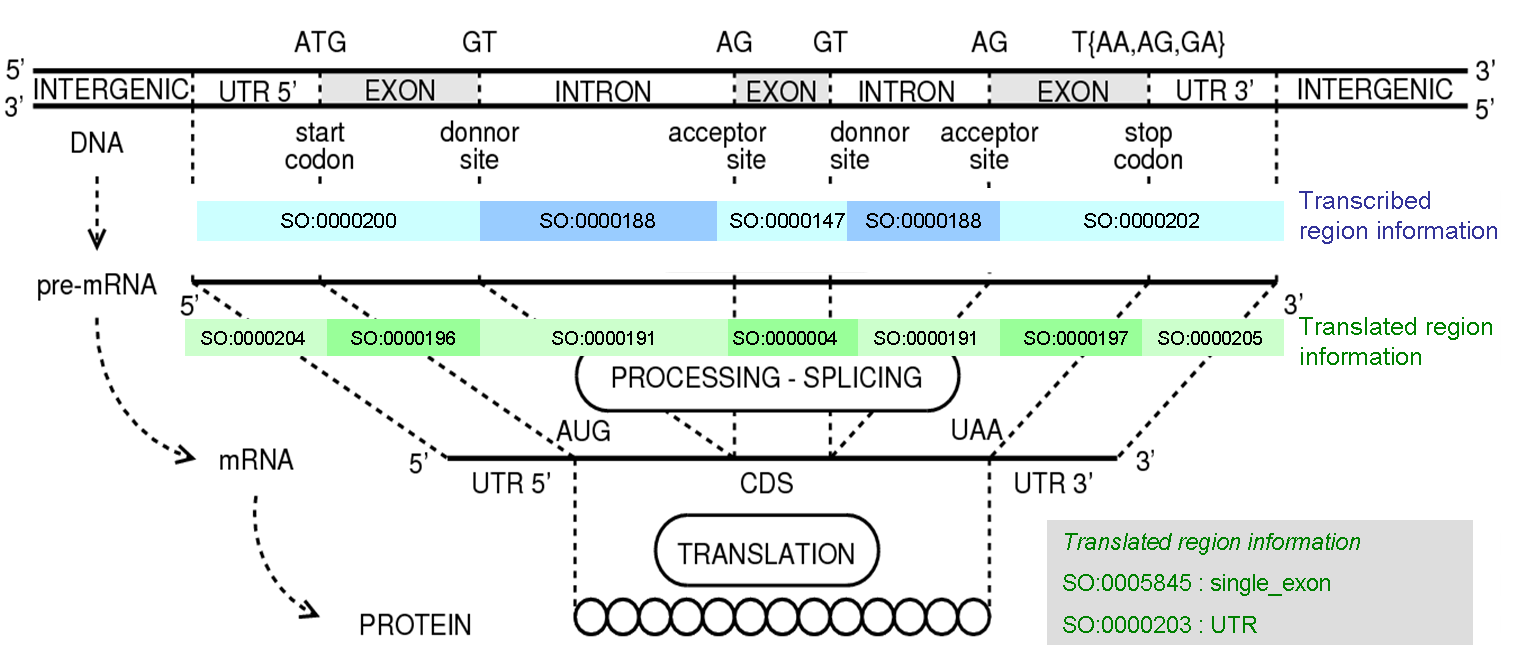
\includegraphics[width=17cm]{SO.png} 
\end{figure}
Here an extract of : seq14ac002535g4g5.tfa.gff.gff3
\begin{Verbatim}[fontsize=\tiny]
seq25	EuGene	five_prime_UTR	1	2787	0	+	.	ID=five_prime_UTR:seq25.0;Ontology_term=SO:0000204
seq25	EuGene	CDS	2788	2836	0	+	0	ID=CDS:seq25.1;Ontology_term=SO:0000196
seq25	EuGene	CDS	8356	8471	0	+	2	ID=CDS:seq25.2;Ontology_term=SO:0000004
seq25	EuGene	CDS	8576	8667	0	+	1	ID=CDS:seq25.3;Ontology_term=SO:0000004
seq25	EuGene	CDS	9006	9061	0	+	0	ID=CDS:seq25.4;Ontology_term=SO:0000004
seq25	EuGene	CDS	9567	9655	0	+	1	ID=CDS:seq25.5;Ontology_term=SO:0000004
seq25	EuGene	CDS	10520	10535	0	+	1	ID=CDS:seq25.6;Ontology_term=SO:0000004
seq25	EuGene	CDS	10896	11134	0	+	1	ID=CDS:seq25.7;Ontology_term=SO:0000004
seq25	EuGene	CDS	11544	12005	0	+	2	ID=CDS:seq25.8;Ontology_term=SO:0000004
seq25	EuGene	CDS	12088	12900	0	+	0	ID=CDS:seq25.9;Ontology_term=SO:0000197
seq25	EuGene	three_prime_UTR	12901	14900	0	+	.	ID=three_prime_UTR:seq25.10;Ontology_term=SO:0000205
\end{Verbatim}

For complete gene, ontology terms for CDS can be added on the fly by the plugin if the GFF3 includes Parent information to a transcript level feature. This feature is typically called "mRNA" or "transcript" in gene finders GFF3 output.
If the \texttt{AnnotaStruct.TranscriptFeature} parameter is set accordingly, then the plugin will identify first, internal, terminal and single exon assuming the CDS features are in increasing position order.

\paragraph{Filtering input information}

No filtering beside syntax checking.

\paragraph{Integration of information}

The underlying graph edges are directly modified as indicated. 

\paragraph{Post analyse}

No post analyse.

\paragraph{Graph}

No plotting.





% Documentation of the IfElse sensor

\subsubsection{\texttt{Sensor.IfElse}}

\paragraph{Description}

This plugin is used to combine the predictions of two existing
plugins. It listens to a first plugin. For each possible predictable
item, if this plugin predicts something then this prediction is used.
If the plugin does not predict anything, then the output of the second
plugin is used.
 
The plugin needs only two parameters to be informed:
\texttt{IfElse.SensorIf} and \texttt{IfElse.SensorElse} which indicate
the names of the two slave plugins. The two slave plugins will be
loaded with an instance number equal to one plus the instance number
of the IfElse sensor itself (allowing for nested IfElse).

Here is an example of IfElse parameters definition which uses the NG2
Sensor if it predicts something or else the SPred sensor.
\begin{Verbatim}[fontsize=\small]
IfElse.SensorIf         NG2
IfElse.SensorElse       SPred
Sensor.IfElse.use       1    # Use IfElse sensor
Sensor.IfElse           1       # Sensor priority
\end{Verbatim}

In this case, since the IfElse is loaded as a first plugin (instance
0), the two slave plugins will be instanciated as instance number
one. The parameters for the 2 plugins must therefore be suffixed by
\texttt{[1]}.

\paragraph{Input files format}

No input files  needed beyond those used by the slave sensors.

\paragraph{Filtering input information}

No filtering.

\paragraph{Integration of information}

The ``If'' plugin is called. For each of the possible information type
(signal and contents), if nothing is predicted by it, the prediction
of the second plugin is used instead.

\paragraph{Post analyse}

No post analyse beyond the post analyze in the slave plugins.

\paragraph{Graph}

Nothing beyond the plotting in the slave plugins.



% Documentation of the Riken sensor

\subsection{\texttt{Sensor.Riken}}

\paragraph{Description}

The plugin allows to exploit 5'/3' EST extracted from the extremities
of full-length cDNA. This type of data was produced by the Riken
institute for Arabidopsis thaliana. By mapping such EST to the genomic
sequence, it is possible to know the positions where a gene
(transcript) must start (5' side) and stop (3' side). The plugin
assumes that this mapping has been done and that the coordinates of
the extremities of the 5' and 3' EST of full-length clones have been
determined before hand.

The sensor is activated by either :
\begin{itemize}
\item the \texttt{-R} argument \index{CmdFlags}{[Riken activation] R}
\item the value TRUE for the parameter \texttt{Sensor.Riken.use} in the
  parameter file.
\end{itemize}

The plugin is controled by several parameters, most of which control
sanity checks (see below). The \texttt{Riken.RAFLPenalty*} parameter
controls the amount of penalty used to force \EuGene\ to predict a
gene on a region defined by a valid EST pair.

Here is an example of Riken parameters definition :
\begin{Verbatim}[fontsize=\small]
Riken.Min_est_diff              100
Riken.Max_overlap               60
Riken.Max_riken_length          60000
Riken.Max_riken_est_length      3000
Riken.Min_riken_length          120 
Riken.Min_riken_est_length      10
Riken.StrandRespect             0
Riken.RAFLPenalty*              -120
Sensor.Riken.use                TRUE     # Use Riken sensor
Sensor.Riken                    7        # Sensor priority
\end{Verbatim}

\paragraph{Input files format}

A file with extension \texttt{.riken} is read.  Each line must contain
the positions of the extremities of the match of the 5' EST then the
name of the 5' EST, the same thing for the 3'EST and finally the name
of the clone.

Here is an exert of a typical \texttt{.riken} file:
\begin{Verbatim}[fontsize=\small]
417757  418379  AV826766        418902  419330  AV796216        0907A18
341382  342036  AU235278        340748  341549  AU225941        1201K23
40318   40969   AV821185        38800   39323   AV781490        0208M10
309757  310341  AV830906        308043  308392  AV813791        0980B11
387624  388227  AU236666        387383  387834  AU227623        1514C21
148345  148909  AV822910        147090  147960  AV783778        0513A17
\end{Verbatim}

\paragraph{Filtering input information}

The plugin uses several parameters that control sanity
checks on the input data.
\begin{itemize}
\item the \texttt{Riken.Max\_riken\_length} parameter controls the
  maximum length for a transcript. If an EST pair defines a transcript
  with a length of more than this number of base pairs, then it is
  ignored. A typical value is 60kb (for \textit{Arabidopsis
    thaliana}).
\item the \texttt{Riken.Min\_riken\_length} parameter controls the
  minimum length for a transcript. If an EST pair defines a transcript
  with a length lower than this number of base pairs, then it is
  ignored. A typical value is 120b (for \textit{Arabidopsis
    thaliana}).
\item the \texttt{Riken.Max\_riken\_est\_length} parameter controls the
  maximum length of the genomic sequence matching one EST. If either
  the 5' or the 3' EST exceed this length, then the EST pair is
  rejected. A typical value is 3kb (for \textit{Arabidopsis
    thaliana}).
\item the \texttt{Riken.Min\_riken\_est\_length} parameter controls the
  minimum length of the genomic sequence matching one EST.  If either
  the 5' or the 3' EST are below this length, then the EST pair is
  rejected. A typical value is 10 bp (for \textit{Arabidopsis
    thaliana}).
\item the \texttt{Riken.StrandRespect} parameter controls whether the
  5'/3' information available for the EST is taken into account or
  ignored. If this parameter is set to \texttt{0}, then the
  information is ignored and the prediction of a gene is ``forced'' in
  the region but with no constraint on the strand.  Otherwise, and if
  the 5'/3' EST pair is separated enough to decide the strand, then
  the prediction of a gene is forced on the strand detected.
\item the \texttt{Riken.Min\_est\_diff} parameter controls the minimum
  distance of separation between the 5' and 3' EST (computed as the
  sum of the distances of the left and right extremities of the two
  genomic sequences mapping the 2 EST) that is sufficient to deduce
  the strand of the gene. A typical value is 100 bp (for
  \textit{Arabidopsis thaliana}).
\item the \texttt{Riken.Max\_overlap} parameter controls how
  information on ``overlapping'' regions is handled. If two EST pairs
  define transcribed regions with a large overlap (larger than the
  parameter value), then it is likely that they refer to the same gene
  (as far as they are detected as being on the same strand). In this
  case, the two EST pairs are taken as one (merged by taking the
  leftmost extremity as the new left extremity and the rightmost as
  the right extremity). If the two overlapping regions are not on the
  same strand, then they are considered as inconsistent and the
  orientation is forgotten.
  
  If the two regions have a small overlap (lower than the parameter
  value), then it is likely that there are 2 different genes with
  overlapping UTR. Because \EuGene\ cannot predict overlapping UTR,
  then the extremities are modified so that they do not overlap
  anymore.
\end{itemize}

\paragraph{Integration of information}

Basically, when a genomic region is validated, the plugin forces
\EuGene\ to predict one single gene in the region. This is done by
penalizing all tracks but the intergenic track just before and after
the gene extremities and by penalizing the intergenic track on the
genomic region itself. If the strand is also considered as detected,
then all tracks on the other strand are also penalized.  Although an
infinite (eg. \texttt{-1e999} in the current double format) penalty
would seem more appropriate, we advocate for a strong finite penalty
to avoid stupid uselss predictions in case of data inconsistency.

\paragraph{Post analyse}

No post analyze.

\paragraph{Graph}

The Riken information is plotted on the output graph as two small
corners delimiting the region on the intergenic track. The corners are
colored differently according to the strand detected for the
transcribed region.






% Documentation of the AnnotaStruct sensor

\subsubsection{\texttt{Sensor.NcRNA}}
\label{ncrna}
\paragraph{Description}

The plugin allows to take into account information from non protein coding RNA. 
For each reading ncRNA region, it rewards the ncRNA tracks, and the ncRNA transcription start and stop signals at the region extemities.

To activate the sensor, put the number of NcRNA instances you want to create to the parameter
\texttt{Sensor.NcRNA.use} in the parameter file.

Here is an example of NcRNA parameters definition:
\begin{Verbatim}[fontsize=\small]
NcRNA.FileExtension[0]  ncrna
NcRNA.NpcRna*[0]        1 
NcRNA.TStartNpc*[0]     1
NcRNA.TStopNpc*[0]      1	
NcRNA.format[0]         GFF3 # Mandatory

Sensor.NcRNA.use        1
Sensor.NcRNA            1
\end{Verbatim}


\paragraph{Gff3 input files format}

The gff3 input mode is activated by setting the value \texttt{GFF3}
for the parameter \texttt{NcRNA.format} in the parameter file.
Note that for the moment, it is mandatory because gff3 is the only reading input format.
The plugin reads its information from the file whose name is the concatenation
of the sequence file name, the \texttt{NcRNA.FileExtension} parameter 
and the \texttt{.gff3} extension.
The accepted features (third column) are:
\begin{itemize}
 \item SO:0000655 or ncRNA
 \item all the terms derived from SO:0000655. For instance, SO:0000252 or rRNA, SO:0000253 or tRNA. 
For details, see  \texttt{http://www.sequenceontology.org/wiki/index.php/Category:} \texttt{SO:0000655\_!\_ncRNA}.
\end{itemize}

If the feature used isn't one of those, the line will be rejected.

Here an extract of \texttt{seq14ac002535g4g5.tfa.ncrna.gff3}:
\begin{Verbatim}[fontsize=\tiny]
seq14	tRNAscan-SE	tRNA	4809	6126	.	+	.	ID=trna:seq14.5;
seq14	tRNAscan-SE	tRNA	7000	7100	.	+	.	ID=trna:seq14.5;
\end{Verbatim}

\paragraph{Filtering input information}

No filtering.

\paragraph{Integration of information}

At each position of a ncRNA region, the ncRNA content edge is reweighted according to the 
\texttt{NcRNA.NpcRna*} parameter value. ncRNA transcription start and stop signals 
are generated at each respective extremity according to the \texttt{NcRNA.TStartNpc*} and \texttt{NcRNA.TStopNpc*} parameter values.


\paragraph{Post analyse}

No post analyse.

\paragraph{Graph}

No plotting.












\subsection{\texttt{Others plugins}}
% Documentation of the GCPlot sensor

\subsection{\texttt{Sensor.GCPlot}}

\paragraph{Description}

The GCPlot sensor allows to add to the graphical representation a plot
of basic composition statistics on the sequence. The sensor is
activated by setting the parameter \texttt{Sensor.GCPlot.use} to
\texttt{TRUE} in the parameter file. The composition statistics
represented can be arbitrarily chosen. For example, the
GC\%=$\frac{G+C}{A+T+G+C}$ is selected by setting \texttt{GCPlot.up}
to \texttt{GC} and \texttt{GCPlot.over} to \texttt{ATGC}. Statistics
on the 3rd base of each codon are automatically computed and plotted.

The color (integer between 0 and 8),, the smoothing window width and a
zooming factor can be specified. The zooming factor for the 3rd base
in each codon in zoomed using specific zooming factor
\texttt{GCPlot.Zoom}

Here is an example of a GCPlot parameter definition :
\begin{Verbatim}[fontsize=\small]
Sensor.GCPlot.use  TRUE      # use GCPlot sensor
Sensor.GCPlot      10        # sensor priority
GCPlot.Up  GC
GCPlot.Over  ATGC
GCPlot.Smooth 98
GCPlot.Color  5    #light green
GCPlot.Zoom 2.0
GCPlot.Zoom3 1.0
\end{Verbatim}

\paragraph{Input files format}

No input file.

\paragraph{Filtering input information}

No filter.

\paragraph{Integration of information}

This sensor does not influence prediction.

\paragraph{Post analyse}

No post analyse.

\paragraph{Graph}

The composition statistics is plotted on the intergenic (IG) track.
The same statistics computed on the 3rd position of each codon is
plotted on the 6 exonic tracks.


% Documentation of the GFF sensor

\subsubsection{\texttt{Sensor.GFF}}

\paragraph{Description}

The GFF sensor allows to add to the graphical representation an
annotation provided in a GFF format. Note that the provided GFF
annotation could be an \EuGene prediction given in GFF format
(obtained using the $-pg$ argument). This could allow to visualise two
predictions on the same graph.

For a sequence, the plugin reads the annotation from one file whose
name is derived from the sequence name by adding the \texttt{.gff}
suffix.  The sensor is activated by either :
\begin{itemize}
\item the \texttt{-G} argument \index{CmdFlags}{[GFF activation] G}
\item the value TRUE for the parameter \texttt{Sensor.GFF.use} in the
  parameter file.
\end{itemize}
Here is an example of GFF parameters definition :
\begin{Verbatim}[fontsize=\small]
Sensor.GFF.use  TRUE      # Use GFF sensor
Sensor.GFF      1         # Sensor priority
\end{Verbatim}

\paragraph{Input files format}

The file \texttt{.gff} describes an annotation for a sequence. The format of
a line is : \texttt{<seqname> <source> <feature> <start> <end> <score>
  <strand> <frame>}. Seqname, source and score fields are ignored.

Example:
\begin{Verbatim}[fontsize=\small]
seqName  EuGene  Utr5    1       199     0       -       .
seqName  EuGene  Utr5    340     359     0       +       .
seqName  EuGene  Init    360     393     0       +       2
seqName  EuGene  Intr    596     732     0       +       0
seqName  EuGene  Intr    830     876     0       +       1
seqName  EuGene  Intr    961     1286    0       +       1
seqName  EuGene  Intr    1396    1478    0       +       2
seqName  EuGene  Intr    1573    1648    0       +       0
seqName  EuGene  Intr    1757    1818    0       +       0
seqName  EuGene  Intr    1962    2057    0       +       2
seqName  EuGene  Intr    2145    2306    0       +       2
seqName  EuGene  Term    2491    2607    0       +       0
seqName  EuGene  Utr3    2608    2626    0       +       .
\end{Verbatim}
Note: only exons are plotted, this file is parsing by the frame field
(no `.' in the frame field).

\paragraph{Filtering input information}

No filter.

\paragraph{Integration of information}

This sensor does not affect prediction.

\paragraph{Post analyse}

No post analyse.

\paragraph{Graph}

Orange horizontal lines are plotted on the exon tracks.


 Documentation of the Plotter sensor

\subsection{\texttt{Sensor.Plotter}}

\paragraph{Description}

The Plotter sensor allows to add to the graphical representation the GC\%,
the GC3\% and the two quotients A/T+A and T/T+A.

The sensor is activated by the value TRUE for the parameter
\texttt{Sensor.Plotter.use} in the parameter file.

Here is an example of Plotter parameters definition :
\begin{Verbatim}[fontsize=\small]
Plotter.GC          1         #
Plotter.GC3         1         # 0 -> no plot  -  1 -> plot
Plotter.A|T/A+T     1         #
Sensor.Plotter.use  TRUE      # Use GFF sensor
Sensor.Plotter      11        # Sensor priority
\end{Verbatim}

\paragraph{Input files format}

No input files  needed.

\paragraph{Filtering input information}

No filtering.

\paragraph{Integration of information}

This sensor does not affect prediction.

\paragraph{Post analyse}

No post analyse.

\paragraph{Graph}

The GC\% is plotted as a thin turquoise line on the intergenic track.
The GC3\% is plotted as a thin turquoise line on each exon tracks.
The T/T+A quotient is plotted as a thin orange line on the forward intron
track.
The A/T+A quotient is plotted as a thin orange line on the reverse intron
track.

% Documentation of the Tester sensor

\subsubsection{\texttt{Sensor.Tester}}

\paragraph{Description}

The Tester sensor allows to evaluate signal sensors. For a sequence,
the plugin reads the truth gene coordinates (note only one complete gene) in GFF format from one file whose name
is derived from the sequence name by adding the \texttt{.gff} suffix.\\
\\
Depending of the value of the parameter \texttt{Tester.Make}, two independant tests could be done. If \texttt{Tester.Make} is set to TEST, the positive positions (where the sensor detects a signal) are analysed (compared to the thruth). The results are written in a file \texttt{test.<sensorName.gff>}. 

If the parameter \texttt{Tester.Make} is set to SPSN, the positions of the canonical coding of the considered signal (ATG for Start; TAG, TAA, TGA for Stop; AG for acceptor; GT, GC for donors) are analysed. Four variables are computed:
\begin{itemize} 
\item TP, number of True Positive
\item FN, number of False Negative
\item FP, number of False Positive
\item TN, number of True Negative
\end {itemize}
With these variables, two others are evaluated:
\begin {itemize}
\item Sn = TP/(TP+FN), sensitivity
\item Sp = TP/(TP+FP), specificity
\end {itemize}

All these variables are computed for all score value given by the sensor. Each value is in turn considered as a threshold (if the score is higher than the threshold the information is considered as positive).\\
The values of the variables are put on stdout. Here is an example.

\begin{Verbatim}[fontsize=\small]
Thres.          Nb      TP      FP      TN      FN      Sens.           Spec.
-3.7297         1       144     16776   230     0       0.851064        100
-3.68888        1       144     16775   231     0       0.851114        100
-3.61192        1       144     16774   232     0       0.851164        100
-3.57555        1       144     16773   233     0       0.851215        100
[...]
\end{Verbatim}
Where Thres. is the threshold value, Nb is the number of observation of the threshold as a score.\\ 
\\ 
To be plotted, specificity and sensibility are also written in the file \texttt{Sensor.<sensorName>.SpSn} and for splice detector sensors only, in the files 
\texttt{Sensor.<sensorName>.Acc} (for acceptor only), \texttt{Sensor.<sensorName>.Don} (for donor only).\\ 
Note that specificity and sensitivity are written in the \texttt{.SpSn}, \texttt{.Acc}, \texttt{.Don} files, only if TP+FP and TP+FN are higher than \texttt{Tester.SPSN.MinNumbers}. This to avoid Sp and Sn based on small effective.\\
\\
The sensor is activated by the value 1 for the parameter
\texttt{Sensor.Tester.use}. A parameter \texttt{Tester.Sensor} indicates which sensor to test. An other parameter \texttt{Tester.Sensor.Instance} defines wich instance (see the 2.2.1 Loading plugins section) of sensor to consider.\\
\\
Here is an example of Tester parameters definition:
\begin{Verbatim}[fontsize=\small]
Tester.Make             SPSN      # SPSN, TEST
Tester.Sensor           EuStop
Tester.Sensor.Instance  0
Tester.SPSN.MinNumbers  100       # greater than 0
Sensor.Tester.use       1      # use Tester sensor
Sensor.Tester           1         # sensor priority
\end{Verbatim}

\paragraph{Input files format}

The file \texttt{.gff} describes the truth coordinates of only one complete gene in GFF format. The format of a
line is :\texttt{<seqname> <source> <feature> <start> <end> <score> <strand> <frame>}. Seqname, source, score and frame fields are ignored.

Example:
\begin{Verbatim}[fontsize=\small]
seqName EuGene  UTR5    866     885     0       +       .
seqName EuGene  E.Init  886     931     0       +       0
seqName EuGene  E.Intr  1014    2366    0       +       1
seqName EuGene  E.Term  2444    2481    0       +       1
seqName EuGene  UTR3    2482    2632    0       +       .
\end{Verbatim}
Note : Feature field must be UTR5, UTR3, E.Init, E.Intr, E.Term or E.Sngl (UTR states are optional).

\paragraph{Output files format}

For the parameter \texttt{Tester.Make} set to TEST, a file
(\texttt{test.<sensorName.gff>}) is created if it does not exist.  For each
predicted signals the Tester sensor write one line in the output file.
The format of this line is : \texttt{<seqname> <source> <feature>
  <score>
  <start> <end> <strand> <frame> <T/F> <state>}.

Where:
\begin{itemize}
\item <seqname> is the 7 first characters of the sequence file name.
\item <source> is the name of the tested sensor.
\item <feature> is the feature type name (can be `Start', `Acc', `Don' and
`Stop').
\item <start> is the predicted signal position.
\item <end> is always `.'.
\item <score> is the score given by the tested sensor.
\item <strand> is `+' for forward and `-' for reverse.
\item <frame> is always `.'.
\item <T/F> is `True' for real site and `False' for the others.
\item <state> is the real state according to the predicted signal
  position (can
  be `IG', `UTR', `ExonF', `ExonR', `IntronF' or `IntronR').
\end{itemize}
Here is an extract of \texttt{test.NG2.gff} :
\begin{Verbatim}[fontsize=\small]
[...]
seqName     NG2     Acc     835       .   -2.26       -       .   False      IG
seqName     NG2     Acc     869       .  -15.03       +       .   False     UTR
seqName     NG2     Acc     918       .  -10.96       -       .   False   ExonF
seqName     NG2     Don     931       .   -0.02       +       .    True   ExonF
seqName     NG2     Don     962       .  -33.06       -       .   False IntronF
seqName     NG2     Don     973       .  -27.76       +       .   False IntronF
seqName     NG2     Don    1011       .   -4.10       -       .   False IntronF
seqName     NG2     Acc    1013       .   -0.10       +       .    True IntronF
seqName     NG2     Acc    1050       .   -7.52       +       .   False   ExonF
seqName     NG2     Don    1050       .  -27.76       +       .   False   ExonF
[...]
\end{Verbatim}

For the parameter \texttt{Tester.Make} set to SPSN, the file \texttt{Sensor.<sensorName>.SpSn} contains on each line a value of specificity and sensitivity for a threshold 
taken from the lowest to the highest.\\ 
For splice detectors sensors, two other files are also written \texttt{Sensor.<sensorName>.Acc} (acceptor only), \texttt{Sensor.<sensorName>.Don} (donor only) with the same format.


\paragraph{Filtering input information}

No filter.

\paragraph{Integration of information}

This sensor does not affect prediction.

\paragraph{Post analyse}

No post analyse.

\paragraph{Graph}

No plot.



\section{\EuGene\ as a combiner}

\EuGene\ is able to integrate predictions from many sources and to combine them in one prediction.
For that, you only need to use the AnnotaStruct plugin (see section~\ref{annotastruct}): create as many AnnotaStruct instances as files to combine.


The parameter file \texttt{cfg/eugene.combine.par} is parametrized to combine two files. 
In the first file, information about start and stop codons is taken into account, whereas in the second one, it is information about splice sites and CDS.
\begin{Verbatim}[fontsize=\small]
 ##### Sensors AnnotaStruct #####
AnnotaStruct.FileExtension[0]      genefinder1
AnnotaStruct.TranscriptFeature[0]  transcript
AnnotaStruct.Start*[0]            2     # i: inline score (GFF3 format only) 
AnnotaStruct.StartType[0]         s      # p: probability  s: score
AnnotaStruct.Stop*[0] 1.5
AnnotaStruct.StopType[0] s
AnnotaStruct.Acc*[0] 0
AnnotaStruct.AccType[0] s
AnnotaStruct.Don*[0] 0
AnnotaStruct.DonType[0] s
AnnotaStruct.TrStart*[0] 0
AnnotaStruct.TrStartType[0] s
AnnotaStruct.TrStop*[0] 0
AnnotaStruct.TrStopType[0] s
AnnotaStruct.Exon*[0] 0
AnnotaStruct.Intron*[0] 0
AnnotaStruct.CDS*[0] 0
AnnotaStruct.format[0]             GFF3
\end{Verbatim}

\begin{Verbatim}[fontsize=\small]
AnnotaStruct.FileExtension[1]      genefinder2
AnnotaStruct.TranscriptFeature[1]  transcript
AnnotaStruct.Start*[1]            0     # i: inline score (GFF3 format only)
AnnotaStruct.StartType[1]          s      # p: probability  s: score
AnnotaStruct.Stop*[1] 0
AnnotaStruct.StopType[1] s
AnnotaStruct.Acc*[1] 3
AnnotaStruct.AccType[1] s
AnnotaStruct.Don*[1] 2.5
AnnotaStruct.DonType[1] s
AnnotaStruct.TrStart*[1] 0
AnnotaStruct.TrStartType[1] s
AnnotaStruct.TrStop*[1] 0
AnnotaStruct.TrStopType[1] s
AnnotaStruct.Exon*[1] 0
AnnotaStruct.Intron*[1] 0
AnnotaStruct.CDS*[1] 4
AnnotaStruct.format[1]             GFF3
#
# SIGNAL/CONTENT SENSORS
Sensor.AnnotaStruct.use 2
#
\end{Verbatim}
More details about AnnotaStruct parameters in the section~\ref{annotastruct}.



\section{Optimization of Plugins parameters}

The value of some numerical plugins parameters (specified in the
parameter file with a name finishing with an '*') can be optimized on
a reference set of sequences (with their related information) for
which genes positions are known. The idea is to adapt the values of
parameters to increase as much as possible the quality of prediction
of genes and exons. The figure \ref{fig:ParaOptimization} details the
general function of the software with input and ouput files.

\begin{figure}[htbp]
  \begin{center}
    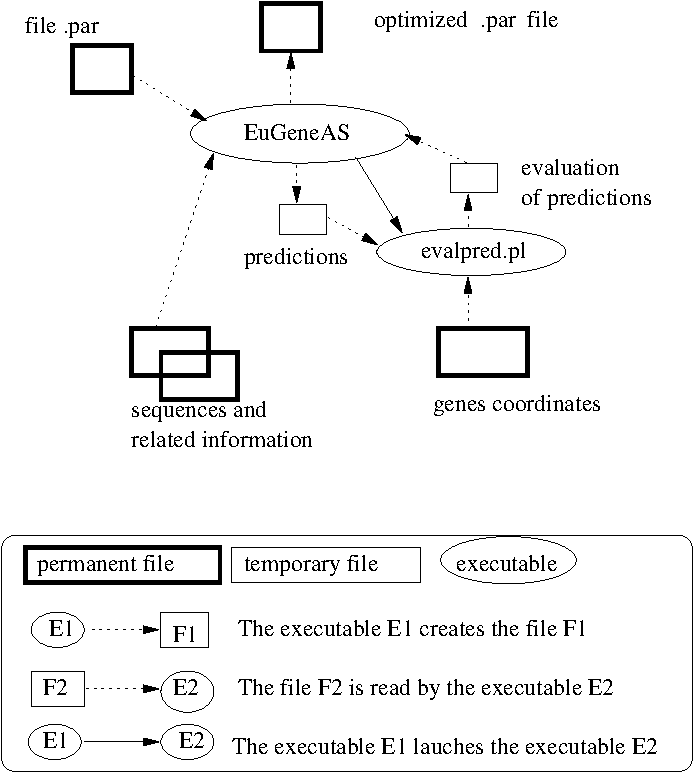
\includegraphics[width=7cm]{ParaOptimization}
  \end{center}
  \caption{Input and output files for parameters optimization} 
  \label{fig:ParaOptimization}
\end{figure}

The optimization can be lauched with the \texttt{-Z} argument
\index{CmdFlags}{[parameters optimization] Z} on the command line or
with the \texttt{ParaOptimi\-zation.Use} parameter set to \texttt{1}.

After updating the parameter file \texttt{eugene.par} (which sensors
to use,...), the software is lauched with the usual command line
specifying as argument the reference sequences to consider. At the
end, the software creates a new parameter file called
\texttt{eugene.<date>.OPTI.par} (for example,
\texttt{eugene.30Sep\-2003.OPTI.par}) with the new value for the
optimized parameters.

For parameters optimization, the inputs to be specified in the
parameter file are:
\begin{itemize}
\item the parameters to optimize with their value domain,
\item the optimization algorithm to use: genetic algorithm, Line
  Search, genetic algorithm and Line Search,
\item the parameters of the optimization algorithm, and for the Line
  Search algorithm complementary information on the parameters to
  optimize (initial value, step of discretization, ...),
\item a file with the coordinates of genes for the sequences set. See below its description.
\item it is possible to include a regulizing term in the criteria
optimized using the \texttt{ParaOptimization.Regularizer} parameter.
The sum of all the absolute values of the parameters multiplied by this parameter is subtracted from the original fitness to define the final fiteness optimized.\end{itemize}

\paragraph{Description of the file with the coordinates of genes}
One line of the file describes one gene. The first field of the line is the sequence name. The followed fields are the list of respectively start and stop positions of the exons of the gene. 
The fields are separated by spaces.
An empty line is required to separate two different sequences.
Note that the order of the sequences is important: the order has to be similar to the result of the 'ls 'command.

Example:
{\scriptsize \begin{verbatim}
SEQ1 429 545 665 750
SEQ1 -2001 -2342 -2424 -2522

SEQ2 1000 1230 1521 1690 2510 2600

\end{verbatim}}
This example describes 2 sequences named SEQ1 et SEQ2. SEQ1 is composed of two genes: the first gene is composed of two exons on the forward strand [429-545] [665-750], 
the second of two exons on the reverse strand [2001-2342] [2424-2522].
SEQ2 has a unique gene composed of three exons [1000-1230] [1521-1690] [2510-2600]

\paragraph{Optimization parameter definition example}
Here is a simplified example of optimization parameters definition in the parameter file. 
{\scriptsize \begin{verbatim}
#################################################################
################### PARAMETERS OPTIMIZATION #####################
#################################################################
ParaOptimization.Use           1
ParaOptimization.Regularizer   0.0
ParaOptimization.TrueCoordFile Araset.coord
ParaOptimization.Algorithm     GENETIC+LINESEARCH
ParaOptimization.Test          FALSE
ParaOptimization.Trace         1
#
ParaOptimization.NbParameter   3
#
ParaOptimization.Para.Name[0]   NStart.startP*
ParaOptimization.Para.Min[0]    0.001
ParaOptimization.Para.Max[0]    15      
#
ParaOptimization.Para.Name[1]   NStart.startB*
ParaOptimization.Para.Min[1]    0.001
ParaOptimization.Para.Max[1]    15      
#
ParaOptimization.Para.Name[2]   EuStop.stopP*
ParaOptimization.Para.Min[2]    0
ParaOptimization.Para.Max[2]    6       
#
################## Genetic ######################################
Genetic.NbRun 2
Genetic.NbGeneration 20
Genetic.NbElement 50
Genetic.Seed 4
Genetic.CrossOverProbability 0.6
Genetic.MutationProbability 0.2
Genetic.SelectionType 1         # 0: roulette wheel 
#                                 1:stochastic remainder without replacement
Genetic.ScalingType 1           # 0: no scaling 
#                                 1: Sigma Truncation scaling 
#                                 2: Power Law scaling
Genetic.Sharing 0.9             # 0: no sharing 
#                                 1: sharing, looking for clusters which best 
#                                    elt fitness is at least n% of the overall 
#                                    best element of the population
Genetic.Clustering 1
Genetic.Elitism 0.9             # 0: none
#                                 n: elitism; keeps the best elt if no sharing,
#                                    and keeps the best elt of each cluster 
#                                    which best_elt fitness is at
#                                    least n% of the overallbest elt if sharing 
Genetic.SA.Mutation FALSE          # Simulated Annealing mutation
Genetic.SA.CrossOver FALSE         # Simulated Annealing crossover
#
#
######### LINESEARCH ###########################################
LineSearch.NbMaxCycle 1
LineSearch.NbMinCycle 1
LineSearch.NbMaxStab 2
LineSearch.DivInter 10
LineSearch.Alpha 0.6
LineSearch.EvolutionMini 0.001
LineSearch.Seed ALEA
#
LineSearch.NbCluster 2
LineSearch.Cluster[0] LINKED
LineSearch.Cluster[1] IDENTICAL
#
LineSearch.Para.Step[0]         0.001
LineSearch.Para.Init[0]         7.5
LineSearch.Para.MinInit[0]      0.001
LineSearch.Para.MaxInit[0]      15
LineSearch.Para.Cluster[0]      0
#
LineSearch.Para.Step[1]         0.001
LineSearch.Para.Init[1]         7.5
LineSearch.Para.MinInit[1]      0.001
LineSearch.Para.MaxInit[1]      15
LineSearch.Para.Cluster[1]      0
#
LineSearch.Para.Step[2]         0.001
LineSearch.Para.Init[2]         3
LineSearch.Para.MinInit[2]      0
LineSearch.Para.MaxInit[2]      6
LineSearch.Para.Cluster[2]      1
#
\end{verbatim} }

\section{Command line flags}
 
\begin{itemize}

\item \texttt{a}: activates the alternative splicing prediction.

\item \texttt{b}: activates the plugin \texttt{Sensor.BlastX}.

\item \texttt{B}: postprocessing activation of the plugin \texttt{Sensor.BlastX}.
  
\item \texttt{c}: controls how successives PNG images overlap (parameter
  \texttt{Output.golap}). It must be followed by the number of
  overlapping nucleotides between 2 successives PNG images. Default is
  heuristically determined based on resolution and number of nuc. per
  image.
 
\item \texttt{d}: activates the plugin \texttt{Sensor.Est}.

\item \texttt{D}: allows to specify a value to a parameter (syntax: -D<para>=<value>).
  \index{CmdFlags}{[eugene parameter definition] D}
  
\item \texttt{E}: enables EST and cDNA post-predition analysis (parameter
  \texttt{Est.PostProcess}) of the Est sensor: after each transcript
  prediction, all matching EST are analyzed and the consistency of the
  EST with the prediction is analyzed. At the end, the number of bases
  of the exon/intron structure predicted which are consistent with at
  least one EST/cDNA are reported.

\item \texttt{f}: the frameshift penalty. A large value prevents
  \EuGene\ from predicting frameshifts (the default).

\item \texttt{g}: graph required.

\item \texttt{G}: activates the plugin \texttt{Sensor.GFF}.

\item \texttt{h}: help \index{CmdFlags}{[eugene help] h}
   
\item \texttt{l}: controls the number of nucleotides that will appear on a
  single image (parameter \texttt{Output.glen}). Default is min
  (6,000 length to visualize). The length to visualize is computed from
  the value given to -u and -v (default is all sequence)
  \index{CmdFlags}{[eugene image size] l}
 
\item \texttt{m}: activates the plugin \texttt{Sensor.MarkovIMM} and specifies 
  the filename of the set of Markov models that will
  be used by the MarkovIMM sensor (parameter \texttt{MarkovIMM.matname}).

\item \texttt{M}:  activates the plugin \texttt{Sensor.MarkovProt} and specifies 
  the filename of the set of Markov models that will
  be used by the MarkovProt sensor (parameter \texttt{MarkovProt.matname}).


\item \texttt{n}: followed by 0 1 or 2. Indicates the way the score are
  normalized accross the possibles states (phase 1,2,3,-1,-2,-3,
  introns and intergenic states). 
  \begin{itemize}
  \item \texttt{0}: no normalization
  \item \texttt{1}: normalize accross all states
  \item \texttt{2}: normalize each coding phase w.r.t. to the non coding
    score only.
  \end{itemize}
  Default is 1 (parameter \texttt{Output.normopt}). Does not affect
  prediction, only text/graphical output.
  \index{CmdFlags}{[eugene graphical score normalization] n}
  
\item \texttt{o}: allows to offset the nucleotide position of the prediction
  (parameter \texttt{Output.offset}).  That is, the prediction for
  nucleotide at position $i$ of the given sequence is printed as
  nucleotide $i+$ the offset. Useful to perform prediction on an
  extracted sequence without loosing the original position.

\item \texttt{O}: allows to specify an output directory (the texttt{Output.Prefix} 
  parameter value).

\item \texttt{p}: controls the format of the textual outpout (parameter
  \texttt{Output.format}). May be d (detailed), l (long), s (short), h
  (html), g (gff) or a (araset format). Default is l.
    
\item \texttt{r}: activates the plugin \texttt{Sensor.Repeat}.

\item \texttt{R}: activates the plugin \texttt{Sensor.Riken}.
  
\item \texttt{s}: forces non partial gene mode prediction. This forbids
  predictions that start and end in intergenic mode and therefore
  prevents the occurrence of partial gene structures on the border of
  the sequence.  Useful if \EuGene\ lacks context around the gene and
  you know a single (or only complete) gene appears on the sequence.
  In practice this simply sets the parameters
  \texttt{EuGene.ExonPrior}, \texttt{EuGene.IntronPrior},
  \texttt{EuGene.FivePrimePrior} and \texttt{EuGene.ThreePrimePrior}
  to $0.0$. \index{CmdFlags}{[eugene non partial gene mode] s}
 
\item \texttt{t}: activates the plugin \texttt{Sensor.Homology}

\item \texttt{u}: controls the part of the sequence whose prediction will be
  displayed in the graphical output (parameter \texttt{Output.gfrom}). It must
  be followed by the position of the 1st nuc. which will be plotted on
  graphical output (allows for zoom'in).  Default is 1.
  
\item \texttt{U}: activates the User information sensor (parameter
  \texttt{Sensor.User.use}). This sensor reads user informations
  stored in .user file. These informations use a small language. The
  language can contain two types of statements. Statements on signals
  (translation start, splice sites) and on the sequence itself
  (coding, non coding...).
  
\item \texttt{v}: controls the part of the sequence whose prediction will be
  displayed in the graphical output (parameter \texttt{Output.gfrom}).
  It must be followed by the position of the last nuc. which will be
  plotted on graphical output (allows for zoom'in). Default is the
  sequence length.
  
\item \texttt{w}: followed by half the size of the smoothing window for the
  scores (parameter \texttt{Output.window}). Default is 48. Does not
  affect prediction, only graphical output.

\item \texttt{x}: controls the horizontal resolution of the PNG images
  generated by EuGene (parameter \texttt{Output.resx}). Default is 900.
  \index{CmdFlags}{[eugene image horizontal resolution] x}
  
\item \texttt{y}: controls vertical resolution of the PNG images generated by
  EuGene (parameter \texttt{Output.resy}).  Default is 400.
  \index{CmdFlags}{[eugene image vertical resolution] y}

\item \texttt{Z}: allows to ask for a parameters optimization (equivallent to
  set the \texttt{ParaOptimization.Use} parameter to 1).
\end{itemize}

\printindex{CmdFlags}{Index of command line flags for sensors}


For more information, have a look to
\textsf{www-bia.inra.fr/T/EuGene}. This gives a rough idea of \EuGene\ 
reliability and the meaning of the graphical output (PDF file, poster
on \EuGene).


\end{document}

